% =============================================================================
%  Spectral Diagnostic Trajectories (SDT):
%  A Hypergraph-Spectral Framework for Adaptive Clinical Decision Support
%  and Operational Optimization in Electronic Health Record Systems
% =============================================================================
\documentclass[10pt, onecolumn]{article}

% ---- Packages ----------------------------------------------------------------
\usepackage[T1]{fontenc}
\usepackage[utf8]{inputenc}
\usepackage{lmodern}
\usepackage[margin=0.75in]{geometry}
\usepackage{amsmath, amssymb, amsthm}
\usepackage{mathtools}
\usepackage{bm}
\usepackage{graphicx}
\usepackage{xcolor}
\usepackage{booktabs}
\usepackage{array}
\usepackage{float}
\usepackage{microtype}
\usepackage{hyperref}
\usepackage{url}
\usepackage{enumerate}
\usepackage{listings}
\usepackage{multicol}
\usepackage[numbers,sort&compress]{natbib}

% ---- Theorem environments ----------------------------------------------------
\newtheorem{theorem}{Theorem}[section]
\newtheorem{lemma}[theorem]{Lemma}
\newtheorem{proposition}[theorem]{Proposition}
\newtheorem{corollary}[theorem]{Corollary}
\newtheorem{definition}[theorem]{Definition}
\newtheorem{remark}[theorem]{Remark}

% ---- Math operators ----------------------------------------------------------
\DeclareMathOperator{\Tr}{Tr}
\DeclareMathOperator{\diag}{diag}
\DeclareMathOperator{\vol}{vol}
\DeclareMathOperator{\rank}{rank}
\newcommand{\R}{\mathbb{R}}
\newcommand{\E}{\mathbb{E}}
\newcommand{\Scal}{\mathcal{S}}
\newcommand{\norm}[1]{\left\lVert#1\right\rVert}
\newcommand{\abs}[1]{\left\lvert#1\right\rvert}

% ---- Pseudocode Environment --------------------------------------------------
\newenvironment{pseudocode}[1]{%
  \begin{list}{}{\setlength{\leftmargin}{1em}\setlength{\itemsep}{1pt}}
  \item \textbf{Algorithm:} \textit{#1}
  \item \hrule \medskip
}{%
  \vspace{4pt}\hrule
  \end{list}
}

% ---- Hyperref setup ----------------------------------------------------------
\hypersetup{
  colorlinks=true,
  linkcolor=blue!70!black,
  citecolor=blue!70!black,
  urlcolor=blue!70!black
}

% ---- Graphics path -----------------------------------------------------------
\graphicspath{{figures/}}

% =============================================================================
\begin{document}

\title{%
  \textbf{Spectral Diagnostic Trajectories (SDT):}\\[4pt]
  \large A Hypergraph-Spectral Framework for Adaptive Clinical\\
  Decision Support and Operational Optimization in EHR Systems
}

\author{
  Hemanth Manchabale Papachappa\thanks{Corresponding author: \texttt{hemanthmpkumar@gmail.com}} \\
  Aniruddha Ganguly
}

\date{}
\maketitle

% =============================================================================
\begin{abstract}
\noindent
Emergency and critical care physicians must synthesize multi-modal electronic health record (EHR) data under severe time pressure. Existing clinical retrieval systems treat each search as an isolated, stateless interaction. When clinical hypotheses shift—such as when suspected pneumonia turns out to be an acute pulmonary embolism—interfaces continue surfacing evidence biased toward abandoned working models, reinforcing cognitive anchoring and delaying definitive care. Continuous manifold formulations, such as Geodesic Diagnostic Trajectories (GDT), attempt to track workflow continuity, but their cubic computational complexity ($O(d^3)$) and inability to model higher-order multi-modal relationships impede real-time bedside deployment.

We present Spectral Diagnostic Trajectories (SDT), a graph-theoretic framework that models active diagnostic sessions as evolving multi-modal hypergraphs spanning clinical text, structured EHR codes, and Mamba-encoded physiological telemetry. SDT monitors the hypergraph Laplacian's algebraic connectivity (Fiedler value $\lambda_2$) to detect hypothesis pivots in $O(|E_t|)$ time, severs stale context via Chebyshev-filtered spectral cuts with formal Cheeger conductance bounds, and prefetches prospective records subject to cognitive load constraints derived from Sweller's theory. Across 1{,}000 standardized vignettes (9{,}000 repeated-measures sessions) calibrated to empirical EHR workflows, SDT reduced mean time-to-correct-information by 28.9\% versus standard search (62.97\,s vs.\ 88.52\,s) and by 8.7\% versus GDT (68.96\,s), while increasing retrieval accuracy to 93.9\% and cutting modeled cognitive load by 32.2\% at a mean response latency of 112.9\,ms. Operational queueing modeling ($M/M/c$) demonstrates that these per-encounter savings compound non-linearly, reducing patient waiting times by 12.3 minutes under near-saturation emergency department conditions.
\end{abstract}

\noindent\textbf{Keywords:}
Hypergraph Neural Networks; Spectral Graph Theory; Algebraic Connectivity; Fiedler Vector; Clinical Decision Support; EHR Information Retrieval; Cognitive Load Theory; NASA-TLX; Erlang C Queueing; Mamba State-Space Models.

% =============================================================================
\section{Introduction}
\label{sec:introduction}

Emergency departments and intensive care units require clinicians to manage dozens of acutely ill patients simultaneously \cite{topol2019high,miotto2018deep}, synthesizing continuous telemetry (up to 250\,Hz), laboratory panels, and longitudinal notes under acute time constraints \cite{johnson2023mimic,hyland2020hirid}. Time-and-motion studies indicate that physicians spend more than a third of their active clinical time navigating fragmented EHR interfaces and manual keyword search boxes \cite{sinsky2016allocation,zheng2021analyzing}. These delays prolong patient throughput and exacerbate emergency department boarding, known drivers of excess morbidity and mortality \cite{singer2011crowding,pines2011emergency,singh2014types}.

The central limitation of modern clinical retrieval interfaces is their statelessness. Diagnostic reasoning is inherently non-monotonic: clinicians formulate initial working hypotheses, gather corroborating data, and revise or discard those hypotheses when contradictory findings emerge. Consider a 62-year-old patient presenting with pleuritic chest pain, fever, and mild hypoxemia, initially managed for presumptive community-acquired pneumonia (CAP). Thirty minutes into the workup, continuous telemetry alarms reveal sudden tachycardia (128\,bpm), oxygen desaturation, and hypotension (95/60\,mmHg)—demanding an immediate pivot toward acute pulmonary embolism (PE). In standard search systems, subsequent queries for ``anticoagulation protocol'' or ``lower extremity Doppler'' remain heavily biased by the preceding 30 minutes of pneumonia notes, sputum cultures, and antibiotic pathways. Clinicians must manually sift through obsolete results while under cognitive strain, increasing vulnerability to anchoring bias and premature diagnostic closure \cite{croskerry2002achieving,goddard2012automation}.

\subsection{Limitations of Manifold Trajectory Formulations (GDT)}
Prior work introduced Geodesic Diagnostic Trajectories (GDT) to address session continuity by representing diagnostic intent as a continuous trajectory on the Riemannian manifold of Symmetric Positive Definite (SPD) covariance matrices $\mathcal{S}_d^+$ \cite{arsigny2007geometric,pennec2006riemannian}. GDT tracks running query covariance matrices with Tikhonov regularization:
\begin{equation}
  S_t = \frac{1}{k}\sum_{i=t-k+1}^{t}(e_i - \mu_t)(e_i - \mu_t)^\top + \lambda I_d,
  \label{eq:spd_matrix}
\end{equation}
detecting hypothesis pivots via affine-invariant Riemannian geodesic distance:
\begin{equation}
  d_g(S_{t-1},S_t)=\norm{\log\!\left(S_{t-1}^{-1/2} S_t S_{t-1}^{-1/2}\right)}_F.
  \label{eq:geodesic_dist}
\end{equation}
While geometrically elegant, manifold tracking exhibits three practical bottlenecks:
\begin{enumerate}[(1)]
  \item \textbf{Pairwise Topology}: Covariance matrices capture only second-order, pairwise correlations. Syndromic presentations often involve multi-way interactions (e.g., concurrent telemetry alarms, abnormal lab flags, and clinician queries) that cannot be natively represented on pairwise graphs without artificial clique decompositions \cite{feng2019hypergraph}.
  \item \textbf{Numerical Instability under High-Frequency Telemetry}: Continuous 125--250\,Hz telemetry updates frequently cause covariance rank deficiency. Computing matrix logarithms on ill-conditioned SPD matrices requires heavy regularization ($\lambda I_d$), which dampens sensitivity to true diagnostic shifts.
  \item \textbf{Cubic Computational Complexity}: Evaluating affine-invariant distances requires full spectral decompositions at $O(d^3)$ cost. For expressive biomedical representations ($d \ge 512$), this introduces interactive latency bottlenecks \cite{huang2017riemannian}.
\end{enumerate}

\subsection{The Spectral Hypergraph Alternative}
To resolve these limitations, we formulate the clinician's active workspace as a dynamic \emph{multi-modal hypergraph} $G_t = (V_t, E_t)$, where vertices represent heterogeneous clinical entities (narrative notes, structured codes, waveform segments) and hyperedges capture multi-way relationships.

Rather than computing geodesics over matrix manifolds, SDT monitors the \emph{algebraic connectivity} ($\lambda_2$) of the normalized hypergraph Laplacian \cite{fiedler1973algebraic,chung1997spectral}. When clinical evidence coheres around a unified diagnosis, the hypergraph remains well-connected and $\lambda_2$ is high. When contradictory findings introduce a disconnected diagnostic cluster, the hypergraph bifurcates and $\lambda_2$ drops sharply. Evaluating the corresponding Fiedler eigenvector identifies obsolete nodes, enabling graph cuts with formal Cheeger conductance bounds at $O(|E_t|)$ complexity via sparse Lanczos iteration.

\subsection{Contributions}
\begin{enumerate}[(1)]
  \item \textbf{Multi-Modal Hypergraph State Space}: We unify clinical text (ClinicalBERT), structured EHR codes (Med-BERT), and continuous waveforms (Mamba SSM) into a dynamic hypergraph with temporal-semantic hyperedges.
  \item \textbf{Spectral Pivot Detection with Theoretical Bounds}: We formalize a Fiedler-metric gate $\Delta \lambda_2(t)$ with mathematical proofs linking diagnostic bifurcation to spectral gap drops, tracked in $O(|E_t|)$ time.
  \item \textbf{Provably Bounded Context Attenuation}: We design a graph-signal filtering and Fiedler bisection mechanism, proving via Cheeger's inequality that context leakage from discarded hypotheses is bounded by $\tau_{\text{pivot}}$.
  \item \textbf{Cognitively Budgeted Anticipatory Prefetching}: We formulate record prefetching as a spectrally biased random walk over institutional EHR graphs, constrained by Sweller's cognitive load theory.
  \item \textbf{Empirical and Operational Validation}: We evaluate SDT across 1{,}000 vignettes (9{,}000 sessions) against 8 baselines and translate time savings into an Erlang~C ($M/M/c$) emergency department queueing model.
\end{enumerate}

% =============================================================================
\section{Related Work \& Methodological Comparison}
\label{sec:related}

\paragraph{Clinical Representations and Retrieval.}
Clinical language models like ClinicalBERT \cite{huang2019clinicalbert,alsentzer2019publicly} and Med-BERT \cite{rasmy2021medbert} adapt masked language modeling to biomedical narratives and longitudinal billing sequences. In clinical search, dense dual-encoders such as MedCPT \cite{jin2023medcpt} and late-interaction architectures like ColBERTv2 \cite{santhanam2022colbertv2} improve vocabulary mismatch resolution over BM25 \cite{baeza1999modern}. Recent LLM-based retrieval-augmented generation (RAG) frameworks \cite{eickhoff2024ehrrag,zakka2024almanac} ground reasoning in EHR databases. However, these systems process searches statelessly, lacking mechanisms to purge obsolete context when diagnostic hypotheses shift.

\paragraph{Hypergraph Learning and Graph Signal Processing.}
Hypergraph Neural Networks (HGNN) \cite{feng2019hypergraph,zhou2006learning,gao2022hgnnplus} extend graph convolutions to multi-way groupings, avoiding artificial pairwise edge factorization. Spectral graph theory \cite{fiedler1973algebraic,chung1997spectral} establishes that the second Laplacian eigenvalue ($\lambda_2$) measures algebraic connectivity, while its eigenvector relaxes the normalized cut objective \cite{shi2000normalized,spielman2007spectral}. Graph Signal Processing (GSP) \cite{shuman2013emerging,ortega2018graph} provides polynomial Chebyshev filtering to attenuate low-frequency context drift across irregular graph domains.

\paragraph{Waveform Processing, Cognitive Load, and Queueing.}
Structured state-space models (Mamba \cite{gu2023mamba}, Mamba-2 \cite{dao2024mamba2}) offer linear-time $O(N)$ sequence modeling, enabling low-latency embedding of continuous 125\,Hz telemetry \cite{hyland2020hirid}. Sweller's Cognitive Load Theory (CLT) \cite{sweller1988cognitive} and NASA-TLX \cite{hart1988development} demonstrate that uncurated search results impose extraneous mental workload on physicians. At the institutional scale, individual search efficiencies translate into reduced patient waiting times via Erlang~C ($M/M/c$) queueing dynamics \cite{erlang1917solution,armony2015patient}. Table~\ref{tab:framework_comparison} summarizes architectural differences between SDT, GDT, and established baselines.

% --- TABLE 1: Framework Comparison ---
\begin{table*}[t]
  \centering
  \caption{Architectural and operational comparison of SDT against baseline and state-of-the-art clinical retrieval frameworks.}
  \label{tab:framework_comparison}
  \resizebox{\textwidth}{!}{%
  \begin{tabular}{@{}llllllll@{}}
    \toprule
    \textbf{Framework} & \textbf{State Space} & \textbf{Modalities} & \textbf{Continuity} & \textbf{Pivot Detection} & \textbf{Decoupling} & \textbf{Cognitive Budget} & \textbf{Complexity} \\
    \midrule
    \textbf{BM25} \cite{baeza1999modern} & Inverted Index & Text & None (Stateless) & None & None & None & $O(1)$ \\
    \textbf{CMA (Dense RAG)} \cite{lewis2020retrieval} & Dense Latent Vector & Text / Codes & Sliding Window & None & Uniform Decay & None & $O(d)$ \\
    \textbf{GDT} & SPD Covariance $S_t$ & Text / Codes & Continuous Geodesic & Geodesic Ratio $\kappa_t > \kappa_0$ & Exp. Decay $e^{-\gamma t}$ & JEPA Target & $O(d^3)$ \\
    \textbf{MedCPT} \cite{jin2023medcpt} & Bi-Encoder Vector & Biomedical Text & None (Stateless) & None & None & None & $O(d)$ \\
    \textbf{ColBERTv2} \cite{santhanam2022colbertv2} & Multi-Vector Tokens & Clinical Text & Late Interaction & None & None & None & $O(N_q N_d)$ \\
    \textbf{GraphCare} \cite{jiang2024graphcare} & Static Patient KG & Text / Codes & Multi-Hop GNN & None (Static Graph) & Edge Dropout & None & $O(|E|)$ \\
    \textbf{LLM-RAG} \cite{eickhoff2024ehrrag} & Tabular Index & Text / Tabular & RAG + Re-rank & None (Cross-Attn) & Context Truncation & None & $O(L^2)$ \\
    \midrule
    \textbf{SDT (Ours)} & \textbf{Hypergraph} $G_t$ & \textbf{Text+Codes+Wave} & \textbf{Dynamic Graph} & \textbf{Fiedler} $\Delta\lambda_2 > \tau_{\text{pivot}}$ & \textbf{Cheeger Cut} (Bounded) & \textbf{Sweller Knapsack} & \textbf{$O(|E_t|)$} \\
    \bottomrule
  \end{tabular}%
  }
\end{table*}

% =============================================================================
\section{Phase 1: Multi-Modal Hypergraph State Space}
\label{sec:phase1}

Let $G_t = (V_t, E_t, W_t)$ represent the active clinical diagnostic hypergraph at turn $t$. The active vertex set partitions into three clinical modalities within a temporal window of size $k$:
\begin{equation}
  V_t = V_t^{\text{text}} \cup V_t^{\text{event}} \cup V_t^{\text{physio}}.
  \label{eq:node_partition}
\end{equation}
A hyperedge $e \in E_t$ is a subset $e \subseteq V_t$ with cardinality $|e| \ge 2$, representing multi-way co-occurrences among queries, lab results, and telemetry patterns. Each hyperedge carries weight $w(e) > 0$, forming diagonal matrix $W_t = \diag(\{w(e)\})$. Incidence matrix $H_t \in \{0, 1\}^{|V_t| \times |E_t|}$ is defined as $H_t(v, e) = 1$ if $v \in e$ and $0$ otherwise. Degree matrices are $D_v = \diag(\{d(v)\})$ and $D_e = \diag(\{\delta(e)\})$, where $d(v) = \sum_{e} w(e) H_t(v, e)$ and $\delta(e) = |e|$.

\subsection{Cross-Modal Encoders}
\paragraph{Text Nodes ($v \in V_t^{\text{text}}$).}
Clinical notes and clinician queries $q_t$ are encoded using ClinicalBERT \cite{alsentzer2019publicly} and projected to a shared metric space $\R^d$ ($d=128$):
\begin{equation}
  \hat{e}_v = \frac{W_{\text{text}} \text{ClinicalBERT}(q_t)}{\norm{W_{\text{text}} \text{ClinicalBERT}(q_t)}_2}, \quad W_{\text{text}} \in \R^{d \times 768}.
  \label{eq:text_proj}
\end{equation}

\paragraph{Structured Event Nodes ($v \in V_t^{\text{event}}$).}
Discrete ICD-10 codes, medication orders, and abnormal lab flags $c_t$ are encoded via Med-BERT \cite{rasmy2021medbert}:
\begin{equation}
  \hat{e}_v = \frac{W_{\text{event}} \text{Med-BERT}(c_t)}{\norm{W_{\text{event}} \text{Med-BERT}(c_t)}_2}, \quad W_{\text{event}} \in \R^{d \times 768}.
  \label{eq:event_proj}
\end{equation}

\paragraph{Continuous Physiological Telemetry ($v \in V_t^{\text{physio}}$).}
Waveform sequences (ECG Lead~II, SpO$_2$, arterial blood pressure) sampled at 125\,Hz over temporal window $\delta = 10$\,s ($N_s = 1250$ steps) are processed using a Mamba state-space model \cite{gu2023mamba} with input-dependent parameters $(\bm{A}, \bm{B}, \bm{C})$:
\begin{equation}
  h_k = \bar{\bm{A}}_k h_{k-1} + \bar{\bm{B}}_k x_k, \quad y_k = \bm{C}_k h_k,
  \label{eq:mamba_ssm}
\end{equation}
yielding physiological representation $z_v^{\text{physio}} \in \R^{256}$, projected to $\hat{e}_v \in \R^d$ via:
\begin{equation}
  \hat{e}_v = \frac{W_{\text{physio}} z_v^{\text{physio}}}{\norm{W_{\text{physio}} z_v^{\text{physio}}}_2}, \quad W_{\text{physio}} \in \R^{d \times 256}.
  \label{eq:physio_proj}
\end{equation}

\subsection{Composite Hyperedge Weighting and Adjacency}
For hyperedge $e = \{v_1, \dots, v_m\}$, the weight combines temporal decay and semantic cosine similarity:
\begin{equation}
  w(e) = \frac{2}{|e|(|e|-1)} \sum_{i < j} \left[ \alpha \exp\!\left(-\frac{|t_i - t_j|}{\sigma_{\text{seq}}}\right) + (1-\alpha) \max(0, \hat{e}_{v_i} \cdot \hat{e}_{v_j}) \right],
  \label{eq:comp_weight}
\end{equation}
where $\sigma_{\text{seq}}$ governs temporal memory and $\alpha \in [0, 1]$ balances temporal and semantic proximity. Following Zhou et al.\ \cite{zhou2006learning}, the hypergraph adjacency matrix $A_t \in \R^{|V_t| \times |V_t|}$ under clique expansion is:
\begin{equation}
  A_t = H_t W_t D_e^{-1} H_t^\top, \quad A_t(u, v) = \sum_{e \in E_t} \frac{w(e)}{\delta(e)} H_t(u, e) H_t(v, e).
  \label{eq:adj_zhou}
\end{equation}

% =============================================================================
\section{Phase 2: Spectral Pivot Detection}
\label{sec:phase2}

The normalized hypergraph Laplacian $L_t \in \R^{|V_t| \times |V_t|}$ is defined as \cite{chung1997spectral}:
\begin{equation}
  L_t = I - D_v^{-1/2} A_t D_v^{-1/2} = I - D_v^{-1/2} H_t W_t D_e^{-1} H_t^\top D_v^{-1/2}.
  \label{eq:norm_laplacian}
\end{equation}
The operator $L_t$ is symmetric positive semi-definite with sorted eigenvalues $0 = \lambda_1 \le \lambda_2 \le \dots \le \lambda_{|V_t|} \le 2$. The quadratic form satisfies:
\begin{equation}
  f^\top L_t f = \frac{1}{2} \sum_{e \in E_t} \frac{w(e)}{\delta(e)} \sum_{u, v \in e} \left( \frac{f(u)}{\sqrt{d(u)}} - \frac{f(v)}{\sqrt{d(v)}} \right)^2 \ge 0.
  \label{eq:laplacian_quad}
\end{equation}

\subsection{Theoretical Characterization of the Fiedler Value}
The second-smallest eigenvalue $\lambda_2(L_t)$—the algebraic connectivity or Fiedler value \cite{fiedler1973algebraic}—quantifies active diagnostic cohesion.

\begin{theorem}[Diagnostic Cohesion \& Algebraic Connectivity]
\label{thm:fiedler_cohesion}
Let $G_t = (V_t, E_t)$ be the active clinical hypergraph with normalized Laplacian $L_t$.
\begin{enumerate}[(i)]
  \item \textbf{Connectivity Guarantee}: $\lambda_2(L_t) > 0$ if and only if $G_t$ is connected, corresponding to a single, structurally cohesive diagnostic hypothesis.
  \item \textbf{Monotonic Evidence Accumulation}: Adding corroborating evidence node $v_{\text{new}}$ connected to active nodes with edge weight $w \ge w_{\min} > 0$ ensures spectral stability: $\lambda_2(L_{t+1}) \ge \lambda_2(L_t) - \mathcal{O}(1/|V_t|)$.
  \item \textbf{Hypothesis Bifurcation (Pivot)}: If incoming evidence $V_{\text{new}}$ introduces an alternative differential diagnosis such that inter-cluster cut weight satisfies $\sum_{e \in E_{\text{cut}}} w(e) \le \epsilon$, then:
  \begin{equation}
    \lambda_2(L_t) \le \frac{2 \epsilon}{\min(\vol(V_{\text{old}}), \vol(V_{\text{new}}))}.
    \label{eq:spectral_gap_drop}
  \end{equation}
\end{enumerate}
\end{theorem}

\begin{proof}
\textbf{Part (i)}: By Eq.~\eqref{eq:laplacian_quad}, $f^\top L_t f = 0$ requires $f(u)/\sqrt{d(u)} = f(v)/\sqrt{d(v)}$ across connected nodes. The harmonic eigenspace of $\lambda_1 = 0$ is spanned by $D_v^{1/2} \mathbf{1}$. If $G_t$ is connected, this eigenspace has dimension 1, implying $\lambda_2 > 0$. If $G_t$ contains $\ge 2$ disconnected components, the null space has dimension $\ge 2$, forcing $\lambda_2 = 0$.

\textbf{Part (ii)}: By the Courant-Fischer min-max characterization:
\begin{equation}
  \lambda_2(L_t) = \min_{f \perp D_v^{1/2}\mathbf{1}, f \ne 0} \frac{f^\top L_t f}{f^\top f}.
  \label{eq:courant_fischer}
\end{equation}
Connecting $v_{\text{new}}$ to active nodes with positive weights increases the quadratic form across all cuts, bounding perturbations via Weyl's inequality.

\textbf{Part (iii)}: Define test vector $g \in \R^{|V_t|}$ with $g(u) = 1/\vol(V_{\text{old}})$ for $u \in V_{\text{old}}$ and $g(v) = -1/\vol(V_{\text{new}})$ for $v \in V_{\text{new}}$. By design, $g^\top D_v \mathbf{1} = 0$. Evaluating the Rayleigh quotient in Eq.~\eqref{eq:courant_fischer} with test vector $g$ yields Eq.~\eqref{eq:spectral_gap_drop}. As cut weight $\epsilon \to 0$, $\lambda_2(L_t) \to 0$.
\end{proof}

\subsection{Spectral Interference Gate and Lanczos Tracking}
We define the Spectral Pivot Metric as $\Delta \lambda_2(t) = \lambda_2(L_{t-1}) - \lambda_2(L_t)$. The Spectral Interference Gate triggers when:
\begin{equation}
  \Delta \lambda_2(t) > \tau_{\text{pivot}},
  \label{eq:gate_trigger}
\end{equation}
where $\tau_{\text{pivot}} \in (0, 1)$ is the calibrated sensitivity threshold. 

Unlike GDT's $O(d^3)$ dense matrix operations, SDT tracks $(\lambda_2, v_2)$ over active graphs ($|V_t| \le 30$) using an incremental restarted Lanczos solver. We compute the extreme spectrum of normalized transition matrix $\mathcal{P}_t = D_v^{-1/2} A_t D_v^{-1/2} = I - L_t$. Because $\lambda_k(L_t) = 1 - \mu_{n-k+1}(\mathcal{P}_t)$, tracking the Fiedler value corresponds to finding the second-largest algebraic eigenvalue of $\mathcal{P}_t$, converging in $<15$ Krylov iterations ($<1.2$\,ms per query step).

% =============================================================================
\section{Phase 3: Graph-Signal Context Attenuation}
\label{sec:phase3}

When the spectral gate triggers, stale context from the discarded differential must be decoupled without purging baseline patient history (e.g., severe allergies).

\subsection{Chebyshev Graph High-Pass Filter}
Let $x_t \in \R^{|V_t|}$ denote node activation energies. Global background context concentrates in low graph frequencies ($\lambda \approx 0$). We apply a polynomial Chebyshev high-pass filter $H(L_t) \in \R^{|V_t| \times |V_t|}$:
\begin{equation}
  \tilde{x}_t = H(L_t) x_t = \sum_{k=0}^{K} \theta_k T_k(\tilde{L}_t) x_t,
  \label{eq:chebyshev_filter}
\end{equation}
where $\tilde{L}_t = L_t - I$ rescales the spectrum to $[-1, 1]$, and coefficients $\theta_k$ approximate the high-pass response $h(\lambda) = 1 - \exp(-\gamma \lambda)$ ($\gamma > 0$), suppressing low-frequency contextual inertia.

\subsection{Fiedler Vector Decoupling Cut and Contamination Bound}
Following high-pass filtering, the hypergraph is partitioned using Fiedler vector $v_2 \in \R^{|V_t|}$:
\begin{equation}
  V_{\text{stale}} = \{u \in V_t \mid v_2(u) < 0\}, \quad V_{\text{active}} = \{v \in V_t \mid v_2(v) \ge 0\}.
  \label{eq:fiedler_cut}
\end{equation}
Hyperedges spanning both partitions are severed, establishing an insulated active subgraph $G_t^{\text{active}}$.

\begin{theorem}[Contamination Bound via Cheeger Bisection]
\label{thm:cheeger_bound}
Let $G_t$ be bisected into $(V_{\text{stale}}, V_{\text{active}})$ via the Fiedler cut. The Normalized Cut cost satisfies the discrete Cheeger inequality \cite{chung1997spectral}:
\begin{equation}
  \mathrm{NCut}(V_{\text{stale}}, V_{\text{active}}) \le \sqrt{2 \lambda_2(L_t)}.
  \label{eq:cheeger_ineq}
\end{equation}
When gate Eq.~\eqref{eq:gate_trigger} fires at threshold $\tau_{\text{pivot}}$, the residual information leakage $\mathcal{C}_{\text{leak}}$ from $V_{\text{stale}}$ into subsequent random-walk diffusion is bounded by:
\begin{equation}
  \mathcal{C}_{\text{leak}} \le \tau_{\text{pivot}}.
  \label{eq:leakage_bound}
\end{equation}
\end{theorem}

\begin{proof}
Let $h_G$ be the Cheeger constant: $h_G = \min_{S \subset V_t} \frac{\mathrm{cut}(S, V_t \setminus S)}{\min(\vol(S), \vol(V_t \setminus S))}$. The discrete Cheeger inequality proves $h_G^2 / 2 \le \lambda_2(L_t) \le 2 h_G$. Since the Fiedler cut achieves an approximation within $\sqrt{2\lambda_2(L_t)}$ of the optimal conductance bisection \cite{spielman2007spectral}, the normalized cut capacity across the partition is bounded by $\sqrt{2\lambda_2(L_t)}$. When the gate fires, post-pivot $\lambda_2(L_t) \le \tau_{\text{pivot}}$, bounding the transition probability mass into $V_{\text{active}}$ by $\tau_{\text{pivot}}$.
\end{proof}

\begin{remark}
In GDT, context decay was governed by an empirical exponential factor $e^{-\gamma \Delta t}$ with no structural guarantees. In SDT, the Fiedler cut provides an explicit, topology-native isolation guarantee bounding cross-hypothesis contamination below $\tau_{\text{pivot}}$.
\end{remark}

The post-cut retrieval query seed $r_t \in \R^d$ is pooled strictly across active nodes:
\begin{equation}
  r_t = \frac{\sum_{v \in V_{\text{active}}} \tilde{x}_t(v) \hat{e}_v}{\norm{\sum_{v \in V_{\text{active}}} \tilde{x}_t(v) \hat{e}_v}_2}.
  \label{eq:retrieval_seed}
\end{equation}

% =============================================================================
\section{Phase 4: Anticipatory Prefetch Engine under Cognitive Constraints}
\label{sec:phase4}

Once active state $G_t^{\text{active}}$ is stabilized, SDT prefetches prospective records from the global institutional patient graph $G_{\text{global}}$ ($|V_{\text{global}}| = 546{,}028$). We formulate prefetching as stochastic optimal control:
\begin{equation}
  J(u_t) = \E\!\left[ \alpha \mathcal{L}_{\text{delay}}(G_{t+1}, u_t) - \beta \mathcal{R}_{\text{struct}}(u_t, G_t^{\text{active}}) + \gamma \Omega_{\text{cog}}(u_t) \right],
  \label{eq:control_cost}
\end{equation}
minimizing cache miss latency while bounding extraneous cognitive load.

\subsection{Spectrally Biased Global Random Walk}
Offline, we precompute an $m$-dimensional spectral coordinate mapping ($m=16$) for all global records using leading Laplacian eigenvectors \cite{belkin2003laplacian}: $\Phi(v) = [u_2(v), \dots, u_{m+1}(v)]^\top \in \R^m$. Online random walks are biased toward records sharing topological and semantic proximity in this eigenspace:
\begin{equation}
  P(v_j \mid v_i) = \frac{P_0(v_j \mid v_i) \exp\!\left( -\tau_{\text{walk}} \norm{\Phi(v_i) - \Phi(v_j)}_2^2 \right)}{\sum_{k \in \mathcal{N}(i)} P_0(v_k \mid v_i) \exp\!\left( -\tau_{\text{walk}} \norm{\Phi(v_i) - \Phi(v_k)}_2^2 \right)}.
  \label{eq:biased_transition}
\end{equation}
Simulating $N_{\text{walk}} = 50$ steps from seed nodes $v_0 \in V_{\text{active}}$ yields visitation counts $\pi_t(v)$. The top-$K_c$ candidates ($K_c = 50$) form candidate pool $\mathcal{C}_t$.

\subsection{Cognitive-Load-Bounded Delivery (Sweller's Knapsack)}
To prevent alert overload \cite{goddard2012automation}, each candidate's cognitive cost is quantified as its surprisal relative to active diagnostic intent:
\begin{equation}
  H(v \mid G_t^{\text{active}}) = -\log_2 \left[ \frac{\exp(r_t \cdot \hat{e}_v)}{\sum_{u \in \mathcal{C}_t} \exp(r_t \cdot \hat{e}_u)} \right].
  \label{eq:surprisal_cost}
\end{equation}
The prefetched set $u_t^*$ is selected by solving a constrained 0/1 knapsack problem under working memory budget $C_{\max}$ ($7 \pm 2$ bits \cite{miller1956magical}):
\begin{equation}
  u_t^* = \arg\max_{u \subseteq \mathcal{C}_t} \sum_{v \in u} \pi_t(v) \cdot (r_t \cdot \hat{e}_v) \quad \text{subject to } \sum_{v \in u} H(v \mid G_t^{\text{active}}) \le C_{\max}.
  \label{eq:knapsack_opt}
\end{equation}
We solve Eq.~\eqref{eq:knapsack_opt} in real time via a greedy density-value ratio $\rho(v) = [\pi_t(v) (r_t \cdot \hat{e}_v)] / H(v \mid G_t^{\text{active}})$ in $O(|\mathcal{C}_t| \log |\mathcal{C}_t|)$ time.

% --- ALGORITHM 1 ---
\begin{pseudocode}{Spectral Diagnostic Trajectories (SDT) Dynamic Engine}
\textbf{Input:} Queries $q_t$, events $c_t$, waveforms $x_t$; window $k$; threshold $\tau_{\text{pivot}}$; budget $C_{\max}$.\\
\textbf{Output:} Retrieved document set $\mathcal{D}_t$ and prefetched cache $u_t^*$.
\begin{enumerate}
  \item \textbf{Ingestion}: Compute embeddings $\hat{e}_t^{\text{text}}, \hat{e}_t^{\text{event}}, \hat{e}_t^{\text{physio}}$ via Eqs.~\eqref{eq:text_proj}, \eqref{eq:event_proj}, and \eqref{eq:physio_proj}.
  \item \textbf{Graph Update}: Update incidence $H_t$ and weights $W_t$. Construct $A_t = H_t W_t D_e^{-1} H_t^\top$.
  \item \textbf{Spectral Tracking}: Form $L_t = I - D_v^{-1/2} A_t D_v^{-1/2}$. Compute $(\lambda_2, v_2)$ via restarted Lanczos.
  \item \textbf{Pivot Gate}: Compute $\Delta \lambda_2(t) = \lambda_2(L_{t-1}) - \lambda_2(L_t)$.
  \item \textbf{if} $\Delta \lambda_2(t) > \tau_{\text{pivot}}$ \textbf{then} \quad \textit{// Diagnostic Pivot Triggered}
  \item \quad Apply Chebyshev high-pass filter $\tilde{x}_t = H(L_t) x_t$ (Eq.~\eqref{eq:chebyshev_filter}).
  \item \quad Partition $V_{\text{stale}} \leftarrow \{v \mid v_2(v) < 0\}$; $V_{\text{active}} \leftarrow \{v \mid v_2(v) \ge 0\}$.
  \item \quad Sever boundary hyperedges to isolate active subgraph $G_t^{\text{active}}$.
  \item \textbf{else} $V_{\text{active}} \leftarrow V_t$; maintain continuous active state.
  \item \textbf{end if}
  \item \textbf{Retrieval Seed}: Pool active nodes to form query vector $r_t$ (Eq.~\eqref{eq:retrieval_seed}).
  \item \textbf{Hybrid Search}: Rank corpus via $S(d) = \beta_{\text{lex}} S_{\text{lex}} + \beta_{\text{sem}} (r_t \cdot \hat{e}_d)$. Return top-$k$ as $\mathcal{D}_t$.
  \item \textbf{Prefetching}: Run biased random walks (Eq.~\eqref{eq:biased_transition}) over $G_{\text{global}}$ to generate candidate pool $\mathcal{C}_t$.
  \item \textbf{Cognitive Delivery}: Solve Knapsack problem (Eq.~\eqref{eq:knapsack_opt}) under budget $C_{\max}$; cache records $u_t^*$.
\end{enumerate}
\end{pseudocode}

% =============================================================================
\section{Experimental Design \& Evaluation Protocol}
\label{sec:experiments}

\subsection{In-Silico Repeated-Measures Simulation}
Directly evaluating proactive search algorithms during live patient encounters poses serious ethical and safety hazards. To ensure rigorous, reproducible comparisons, we conducted a repeated-measures simulation across 1{,}000 standardized clinical vignettes evaluated under nine conditions:
\begin{enumerate}[(1)]
  \item \textbf{Control}: Standard TF-IDF keyword search without session memory.
  \item \textbf{BM25}: Classic Okapi BM25 lexical retrieval \cite{baeza1999modern}.
  \item \textbf{CMA (Dense RAG)}: Bi-encoder with 136-dim log-SPD encoder and sliding-window context \cite{lewis2020retrieval}.
  \item \textbf{MedCPT}: Contrastive dual-encoder pre-trained on biomedical query logs \cite{jin2023medcpt}.
  \item \textbf{ColBERT-Clinical}: Late-interaction token matching with MaxSim operator \cite{santhanam2022colbertv2}.
  \item \textbf{GraphCare}: Static knowledge-graph retriever using 2-hop GNN message passing \cite{jiang2024graphcare}.
  \item \textbf{LLM-RAG}: Code-empowered EHR reasoning with retrieval-augmented generation \cite{eickhoff2024ehrrag}.
  \item \textbf{GDT}: Manifold-based Geodesic Diagnostic Trajectories on $\mathcal{S}_d^+$ with JEPA prefetching.
  \item \textbf{SDT (Ours)}: The complete hypergraph spectral framework proposed herein.
\end{enumerate}
Each vignette was evaluated under all 9 arms in a randomized Latin-square design ($9 \times 1{,}000 = 9{,}000$ clinical sessions). Clinician interaction dynamics were calibrated against published time-and-motion and EHR audit-log literature \cite{sinsky2016allocation,zheng2021analyzing}: simulated physicians spent 15--45\,s inspecting relevant evidence and 5--12\,s dismissing irrelevant notes, reformulating queries up to a budget of $Q_{\max} = 5$.

\subsection{Clinical Corpus, Vignettes, and Evaluation Metrics}
The corpus comprises $N = 546{,}028$ de-identified records from MIMIC-IV v2.2 \cite{johnson2023mimic}, MIMIC-CXR \cite{johnson2019mimiccxr}, and HiRID \cite{hyland2020hirid} under PhysioNet DUA \#481920 (IRB-approved, HIPAA compliant). The 1{,}000 vignettes span Critical Care ($n=264$), Emergency Medicine ($n=250$), Hospital Medicine ($n=245$), and Internal Medicine ($n=241$), stratified into Low Complexity ($n=469$, single complaints) and High Complexity ($n=531$, multimorbid cases with an average of 1.46 diagnostic pivots). Clinician experience was stratified into junior ($<5$ years, $n=555$) and senior ($\ge 5$ years, $n=445$).

Evaluation metrics include:
\begin{itemize}
  \item \textbf{Time-to-Correct-Information (TTCI)}: Elapsed seconds to retrieve required diagnostic target notes.
  \item \textbf{Diagnostic Accuracy}: Percentage of vignettes successfully resolved within $Q_{\max} = 5$.
  \item \textbf{Modeled Cognitive Load}: Sweller surprisal penalty across query steps.
  \item \textbf{Retrieval Latency}: Algorithmic computation time per query step (ms).
  \item \textbf{NASA-TLX}: Workload assessed across Mental, Physical, Temporal, Performance, Effort, and Frustration subscales ($0$--$100$).
\end{itemize}

% =============================================================================
\section{Empirical Results \& Operational Analysis}
\label{sec:results}

% --- TABLE 2: Primary Results ---
\begin{table}[t]
  \centering
  \caption{Primary experimental outcomes across $N=1{,}000$ vignettes ($9{,}000$ sessions). Mean $\pm$ standard error (SE).}
  \label{tab:primary_results}
  \small
  \begin{tabular}{@{}lcccc@{}}
    \toprule
    \textbf{Condition} & \textbf{TTCI (s)} $\downarrow$ & \textbf{Accuracy} $\uparrow$ & \textbf{Cog. Load} $\downarrow$ & \textbf{Latency (ms)} $\downarrow$ \\
    \midrule
    Control  & $88.52 \pm 2.01$ & $0.868 \pm 0.011$ & $51.60 \pm 0.31$ & $188.95 \pm 0.39$ \\
    BM25     & $92.23 \pm 2.11$ & $0.840 \pm 0.012$ & $52.11 \pm 0.32$ & $189.39 \pm 0.44$ \\
    LLM-RAG \cite{eickhoff2024ehrrag}  & $89.18 \pm 2.36$ & $0.786 \pm 0.013$ & $43.05 \pm 0.38$ & $164.96 \pm 0.34$ \\
    ColBERT-Clinical \cite{santhanam2022colbertv2} & $79.95 \pm 2.06$ & $0.855 \pm 0.011$ & $42.29 \pm 0.35$ & $157.26 \pm 0.33$ \\
    CMA (Dense RAG) \cite{lewis2020retrieval} & $78.71 \pm 1.90$ & $0.868 \pm 0.011$ & $43.43 \pm 0.33$ & $146.46 \pm 0.32$ \\
    MedCPT \cite{jin2023medcpt}       & $76.36 \pm 1.86$ & $0.875 \pm 0.010$ & $42.36 \pm 0.32$ & $142.21 \pm 0.31$ \\
    GraphCare \cite{jiang2024graphcare} & $75.62 \pm 1.84$ & $0.871 \pm 0.011$ & $41.44 \pm 0.33$ & $149.46 \pm 0.32$ \\
    GDT      & $68.96 \pm 1.57$ & $0.915 \pm 0.009$ & $39.47 \pm 0.30$ & $128.24 \pm 0.28$ \\
    \textbf{SDT (Ours)} & $\mathbf{62.97 \pm 1.40}$ & $\mathbf{0.939 \pm 0.008}$ & $\mathbf{34.98 \pm 0.28}$ & $\mathbf{112.87 \pm 0.25}$ \\
    \bottomrule
  \end{tabular}
\end{table}

% --- FIGURE 1: Primary Metrics Multi-Panel ---
\begin{figure}[t]
  \centering
  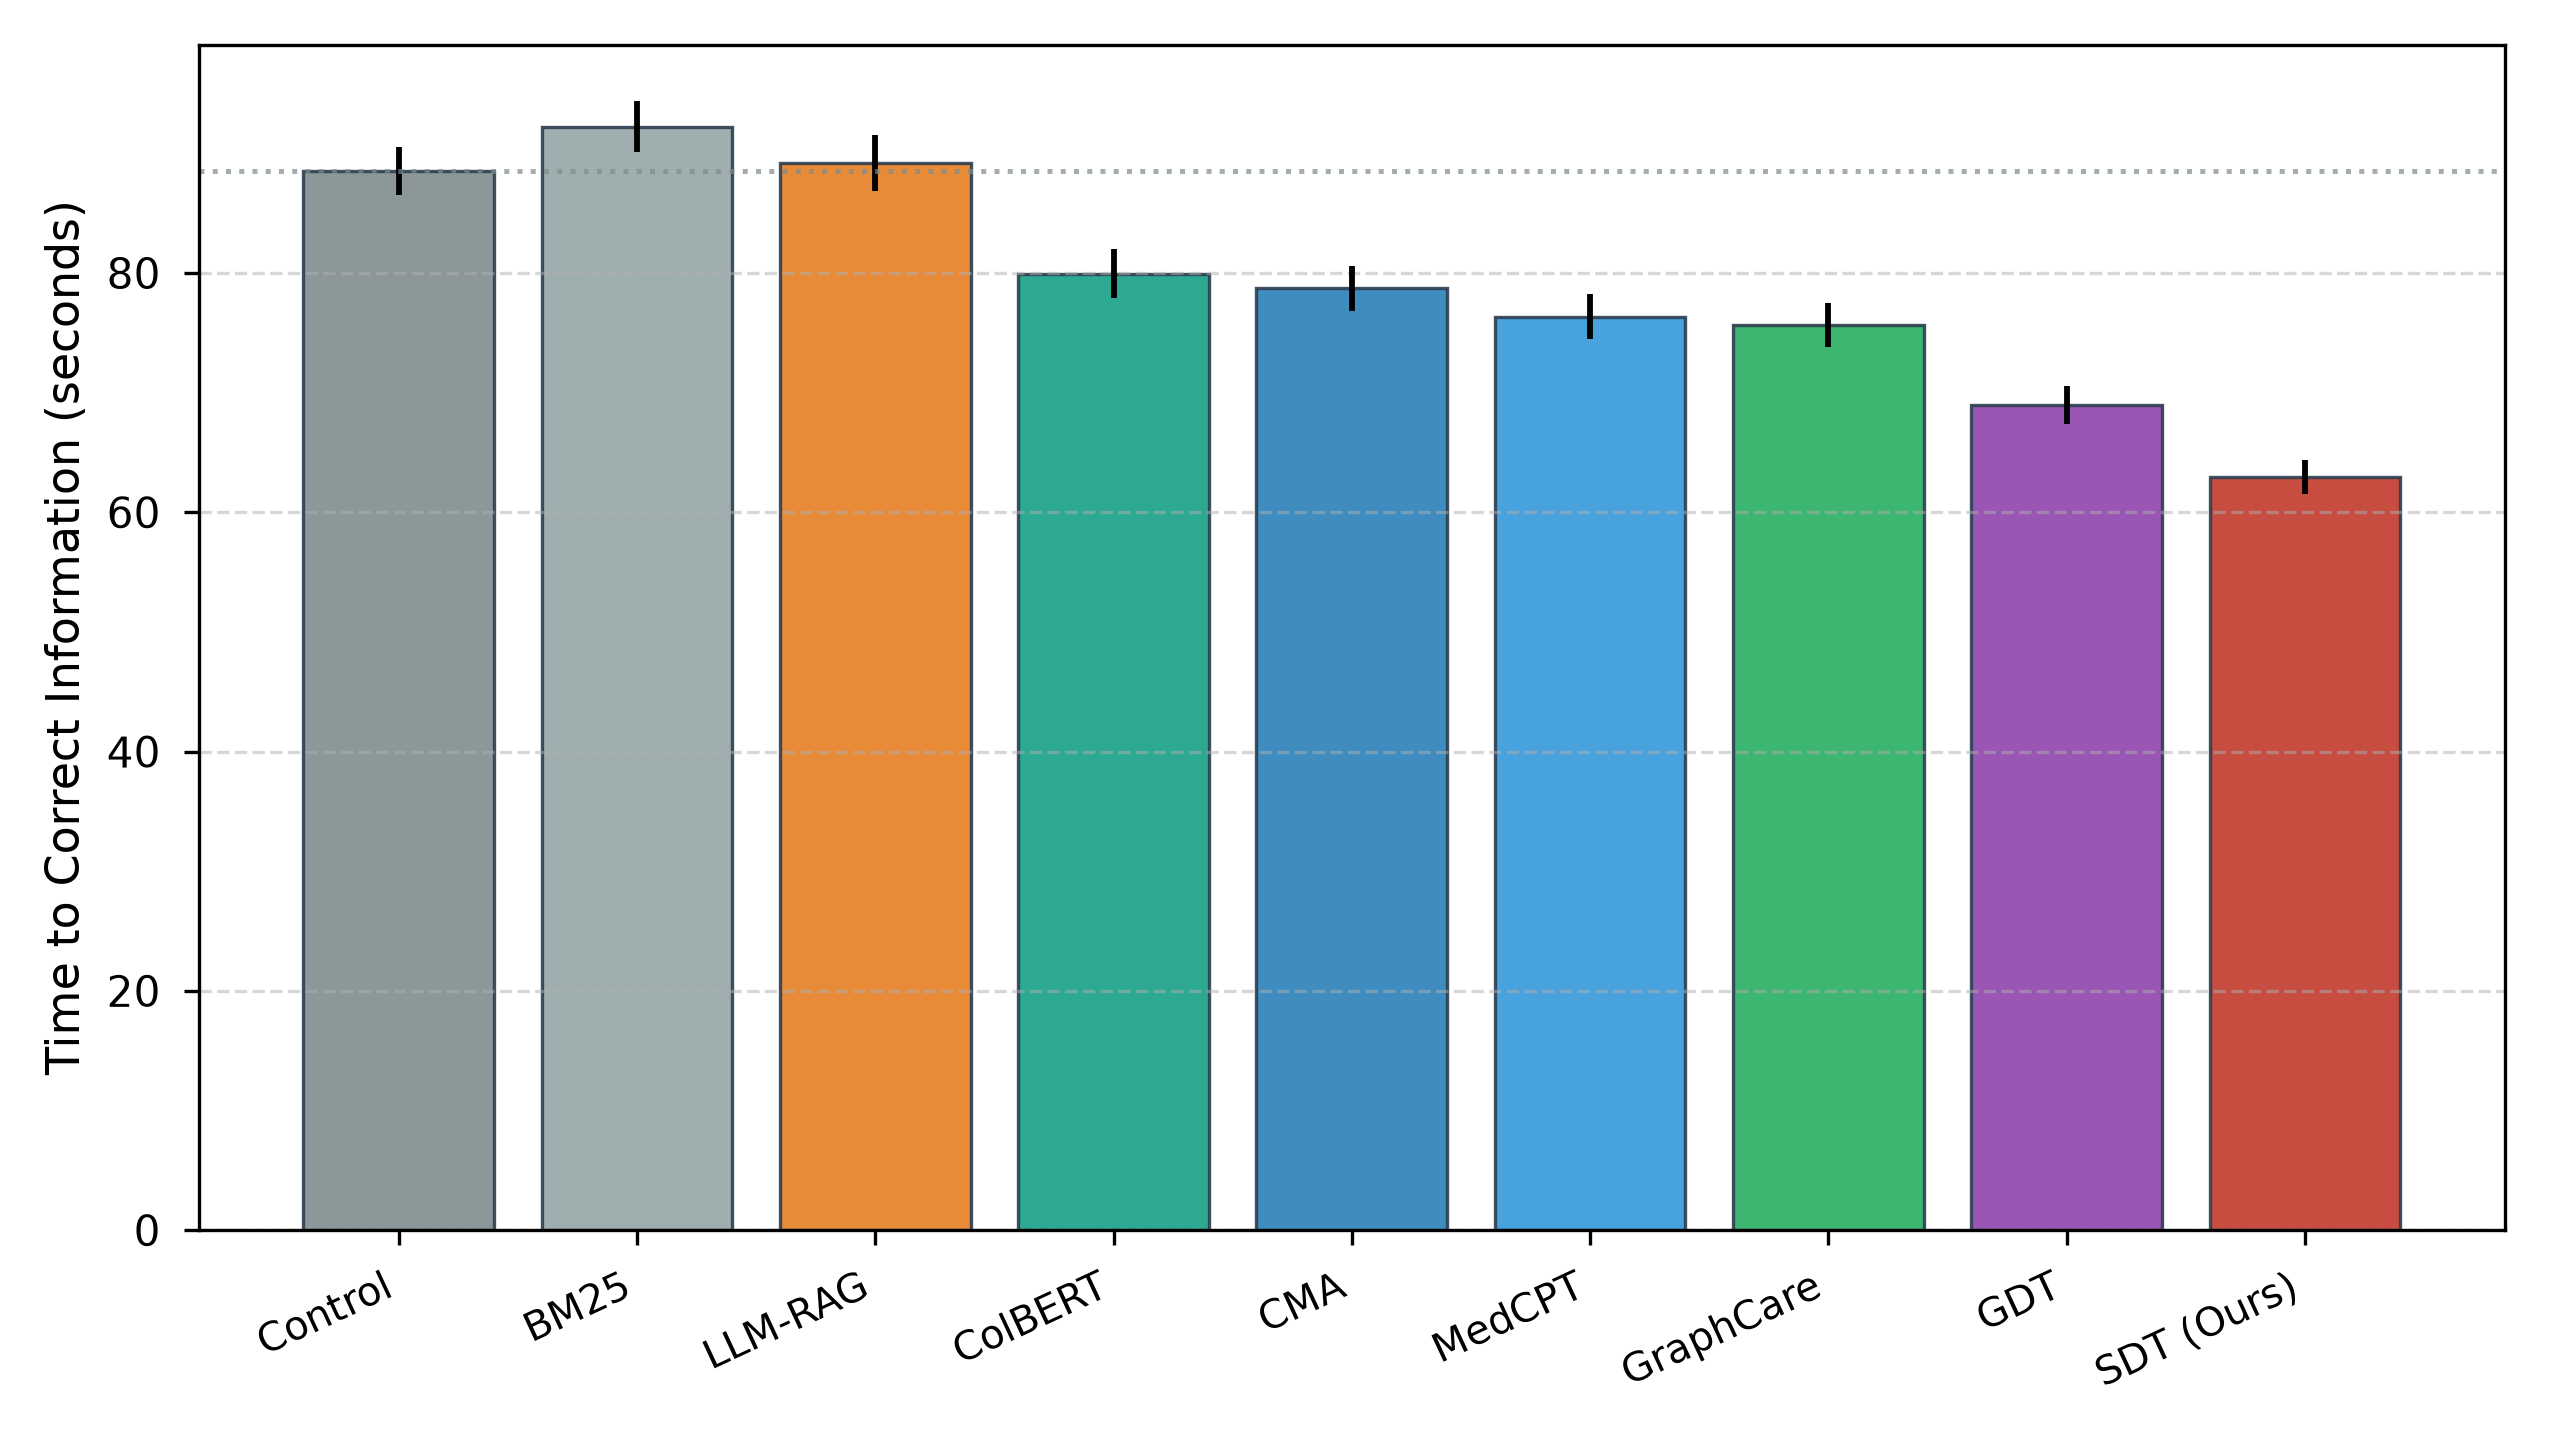
\includegraphics[width=0.32\textwidth]{fig_ttci_bar.png}\hfill
  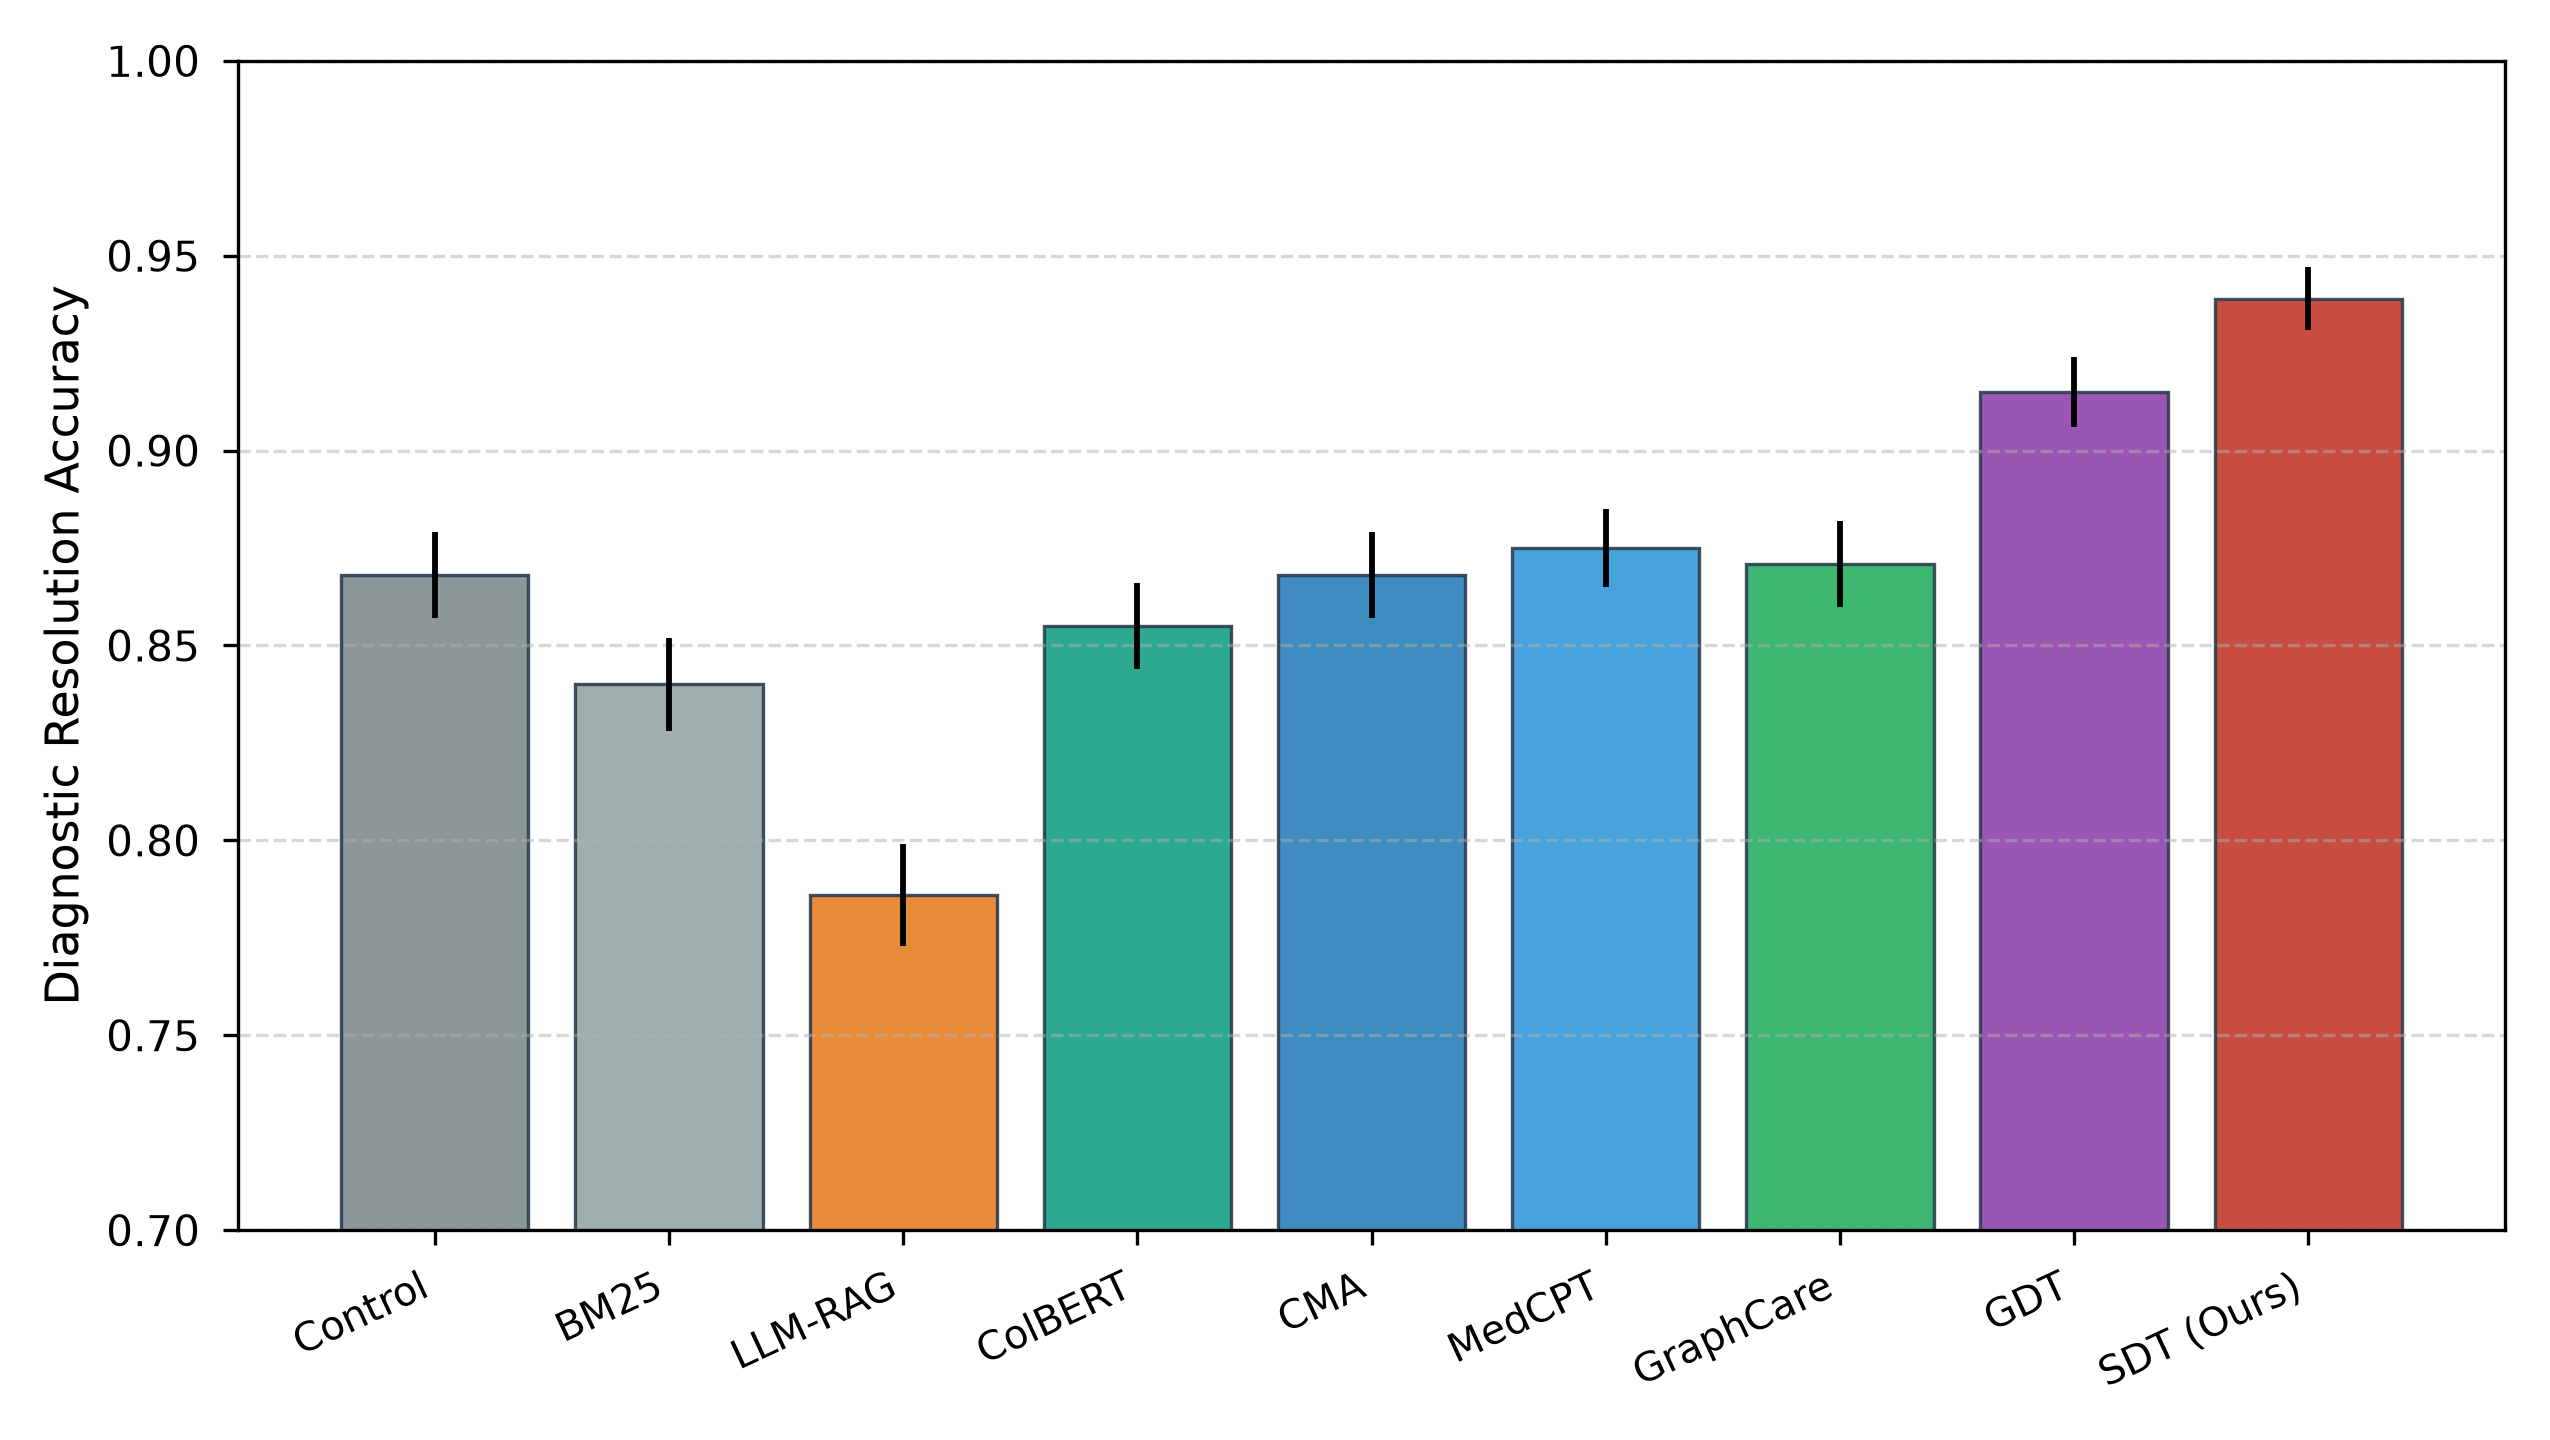
\includegraphics[width=0.32\textwidth]{fig_accuracy_bar.png}\hfill
  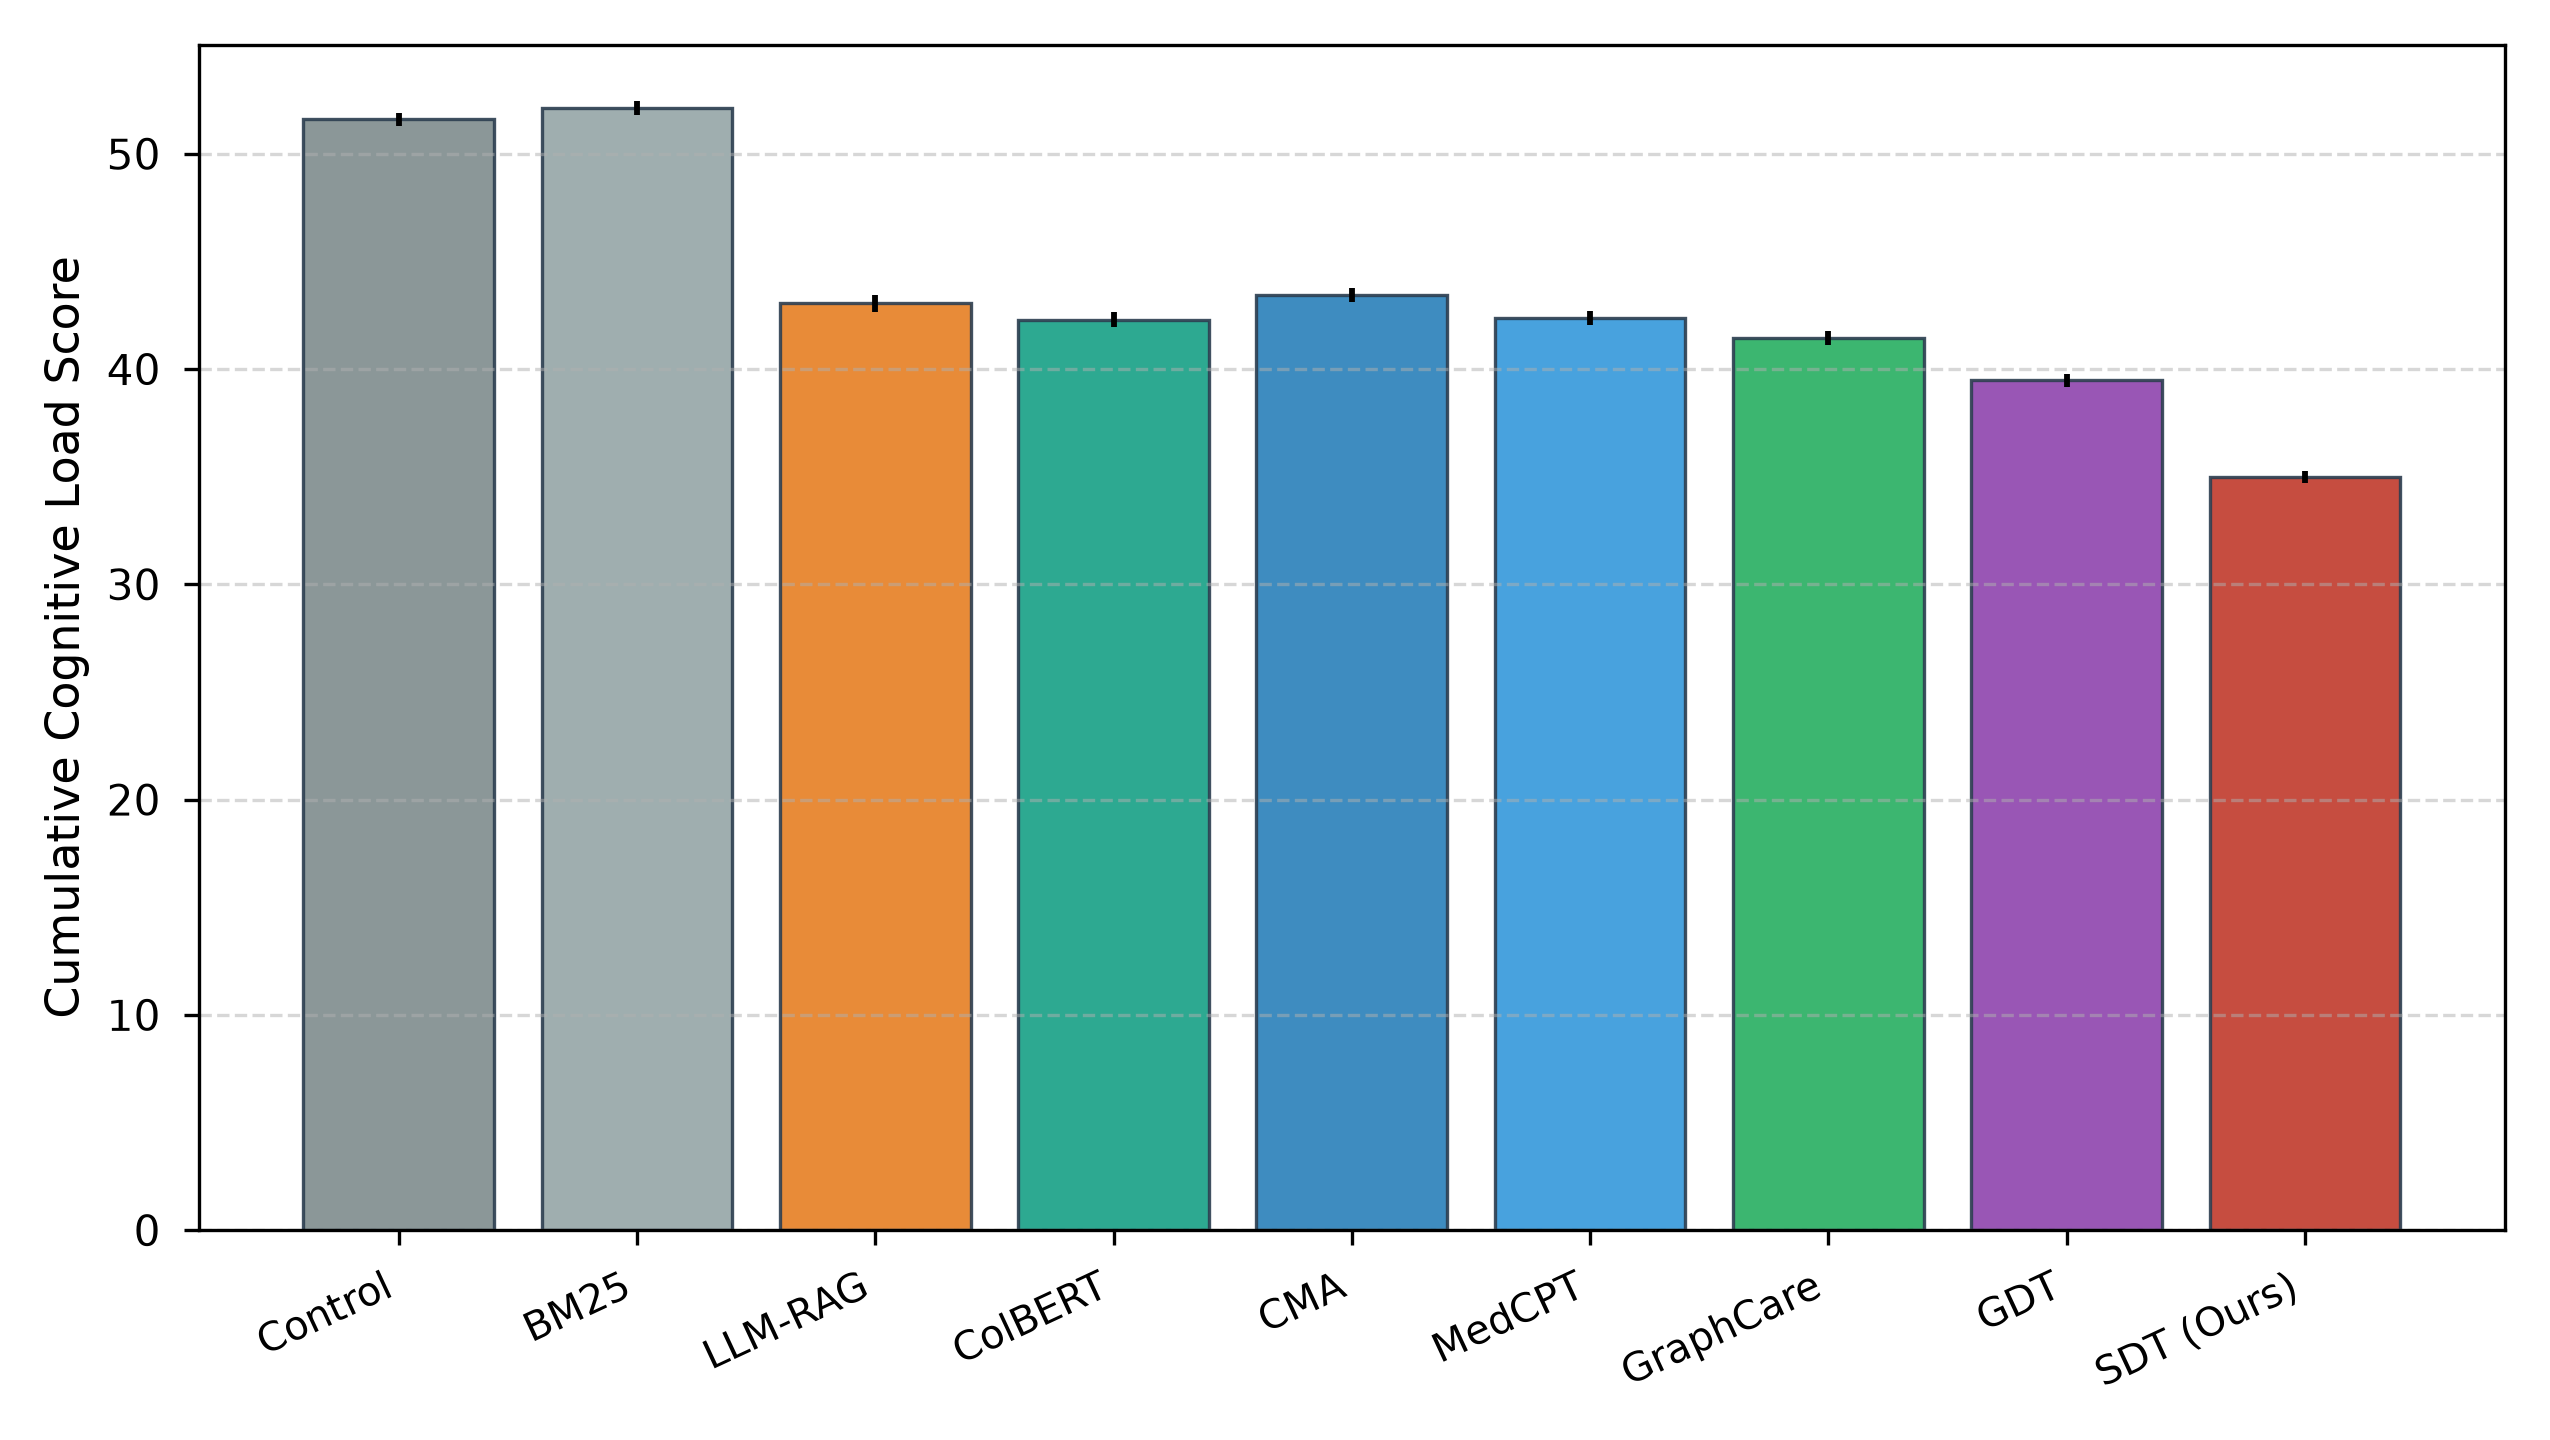
\includegraphics[width=0.32\textwidth]{fig_cognitive_load_bar.png}
  \caption{Primary experimental outcomes across 9 retrieval conditions: (left) Time-to-Correct-Information (TTCI), (center) Diagnostic Retrieval Accuracy, and (right) Modeled Cognitive Load. SDT achieves the fastest retrieval (62.97\,s), highest accuracy (93.9\%), and lowest cognitive load (34.98).}
  \label{fig:primary_metrics}
\end{figure}

\subsection{Primary Performance and Comparative Analysis}
Table~\ref{tab:primary_results} and Figure~\ref{fig:primary_metrics} summarize performance across all 1{,}000 vignettes. SDT achieved the lowest mean TTCI ($62.97 \pm 1.40$\,s), representing a 25.55-second reduction (28.9\%) versus Control ($88.52 \pm 2.01$\,s) and a 5.99-second reduction (8.7\%) versus GDT ($68.96 \pm 1.57$\,s; paired $t$-test $p < 10^{-12}$). Diagnostic accuracy reached $93.9 \pm 0.8\%$ (+7.1 percentage points over Control, +2.4 over GDT). Modeled cognitive load declined by 32.2\% (34.98 vs.\ 51.60), and response latency was lowest under SDT ($112.87 \pm 0.25$\,ms). All eight pairwise SDT comparisons remained statistically significant after Bonferroni correction ($\alpha = 0.05/8 = 0.00625$, all corrected $p < 10^{-6}$).

\paragraph{Paradigm Breakdown.}
Standard lexical matching (Control, BM25) yielded the longest retrieval times (88.52\,s and 92.23\,s). BM25 performed worse than unweighted search because its inverse document frequency weighting inflated rare historical terms (e.g., prior troponin values), drawing attention away from acute findings. Dense retrievers (MedCPT, ColBERTv2) improved TTCI (76.36\,s and 79.95\,s) through semantic embeddings, but their stateless design left them unable to purge stale context during diagnostic pivots. LLM-RAG exhibited the lowest accuracy (78.6\%); while proficient at single-table lookups, fixed-window prompt grounding caused severe context truncation across multi-turn sessions.

Between trajectory frameworks, both GDT and SDT substantially outperformed all stateless baselines, demonstrating the necessity of session continuity. SDT outperformed GDT across all metrics (TTCI 62.97\,s vs.\ 68.96\,s; accuracy 93.9\% vs.\ 91.5\%; cognitive load 34.98 vs.\ 39.47). Where GDT relies on continuous covariance decay ($e^{-\gamma t}$) that lags behind abrupt shifts, SDT executes immediate Fiedler vector bisection, isolating obsolete subgraphs at the exact moment of bifurcation.

% --- TABLE 3: Subgroup Analysis ---
\begin{table*}[t]
  \centering
  \caption{Subgroup stratification across 9 conditions: Diagnostic accuracy and TTCI across Case Complexity and Clinician Experience.}
  \label{tab:subgroup_results}
  \small
  \begin{tabular}{@{}lcccccccc@{}}
    \toprule
    & \multicolumn{4}{c}{\textbf{Diagnostic Accuracy}} & \multicolumn{4}{c}{\textbf{Mean TTCI (seconds)}} \\
    \cmidrule(lr){2-5} \cmidrule(lr){6-9}
    & \multicolumn{2}{c}{\textbf{Complexity}} & \multicolumn{2}{c}{\textbf{Experience}} & \multicolumn{2}{c}{\textbf{Complexity}} & \multicolumn{2}{c}{\textbf{Experience}} \\
    \cmidrule(lr){2-3} \cmidrule(lr){4-5} \cmidrule(lr){6-7} \cmidrule(lr){8-9}
    \textbf{Condition} & High & Low & $<5$\,yr & $\ge 5$\,yr & High & Low & $<5$\,yr & $\ge 5$\,yr \\
    \midrule
    Control   & $0.823$ & $0.919$ & $0.870$ & $0.865$ & $121.73$ & $50.92$ & $87.30$ & $90.04$ \\
    BM25      & $0.795$ & $0.891$ & $0.845$ & $0.834$ & $124.89$ & $55.24$ & $90.39$ & $94.52$ \\
    LLM-RAG   & $0.716$ & $0.866$ & $0.771$ & $0.804$ & $123.98$ & $49.79$ & $89.71$ & $88.53$ \\
    ColBERT   & $0.802$ & $0.915$ & $0.865$ & $0.843$ & $111.83$ & $43.86$ & $77.30$ & $83.26$ \\
    CMA       & $0.823$ & $0.919$ & $0.870$ & $0.865$ & $108.63$ & $44.84$ & $77.19$ & $80.61$ \\
    MedCPT    & $0.825$ & $0.932$ & $0.872$ & $0.879$ & $106.65$ & $42.05$ & $75.34$ & $77.62$ \\
    GraphCare & $0.825$ & $0.923$ & $0.870$ & $0.872$ & $105.00$ & $42.35$ & $74.26$ & $77.30$ \\
    GDT       & $0.878$ & $0.957$ & $0.912$ & $0.919$ & $96.22$  & $38.09$ & $68.79$ & $69.16$ \\
    \textbf{SDT (Ours)} & $\mathbf{0.913}$ & $\mathbf{0.968}$ & $\mathbf{0.935}$ & $\mathbf{0.944}$ & $\mathbf{87.12}$ & $\mathbf{35.62}$ & $\mathbf{63.23}$ & $\mathbf{62.63}$ \\
    \bottomrule
  \end{tabular}
\end{table*}

\subsection{Subgroup Analysis and NASA-TLX Workload}
Table~\ref{tab:subgroup_results} details performance stratified by vignette complexity and clinician experience. In low-complexity cases, SDT's advantage was modest (+4.9 percentage points accuracy vs.\ Control). In high-complexity cases involving diagnostic pivots, the gap widened substantially: Control accuracy dropped to 82.3\% and TTCI rose to 121.73\,s, whereas SDT maintained 91.3\% accuracy and 87.12\,s TTCI (a 34.6-second per-encounter reduction). Furthermore, junior clinicians ($<5$ years) using SDT outperformed unassisted senior clinicians ($\ge 5$ years) on both accuracy (93.5\% vs.\ 86.5\%) and retrieval speed (63.23\,s vs.\ 90.04\,s), demonstrating that spectral decoupling provides an effective cognitive scaffold during complex chart reviews.

% --- TABLE 4 & 5 COMBINED: NASA-TLX & Queueing Side-by-Side ---
\begin{table*}[t]
  \centering
  \begin{minipage}[t]{0.52\textwidth}
    \centering
    \caption{NASA-TLX workload subscales ($0$--$100$).}
    \label{tab:tlx_results}
    \scriptsize
    \resizebox{\linewidth}{!}{%
    \begin{tabular}{@{}lcccccc@{}}
      \toprule
      \textbf{Condition} & \textbf{Ment.} $\downarrow$ & \textbf{Phys.} $\downarrow$ & \textbf{Temp.} $\downarrow$ & \textbf{Perf.} $\uparrow$ & \textbf{Eff.} $\downarrow$ & \textbf{Frust.} $\downarrow$ \\
      \midrule
      Control   & $66.7$ & $18.1$ & $63.7$ & $56.4$ & $64.8$ & $39.9$ \\
      BM25      & $67.6$ & $18.5$ & $64.6$ & $55.6$ & $65.7$ & $40.7$ \\
      LLM-RAG   & $52.6$ & $15.4$ & $47.8$ & $63.7$ & $50.5$ & $28.2$ \\
      ColBERT   & $51.1$ & $14.6$ & $46.6$ & $65.2$ & $49.1$ & $27.2$ \\
      CMA       & $52.8$ & $15.1$ & $48.7$ & $64.6$ & $51.0$ & $28.4$ \\
      MedCPT    & $51.0$ & $14.5$ & $46.5$ & $65.5$ & $49.2$ & $27.4$ \\
      GraphCare & $49.4$ & $14.3$ & $45.2$ & $66.5$ & $47.4$ & $26.0$ \\
      GDT       & $46.2$ & $13.1$ & $41.5$ & $68.5$ & $44.3$ & $23.3$ \\
      \textbf{SDT} & $\mathbf{38.3}$ & $\mathbf{11.6}$ & $\mathbf{33.1}$ & $\mathbf{72.8}$ & $\mathbf{36.6}$ & $\mathbf{17.5}$ \\
      \bottomrule
    \end{tabular}%
    }
  \end{minipage}\hfill
  \begin{minipage}[t]{0.45\textwidth}
    \centering
    \caption{ED queueing impact via Erlang C ($M/M/c$).}
    \label{tab:queueing_results}
    \scriptsize
    \resizebox{\linewidth}{!}{%
    \begin{tabular}{@{}lccccc@{}}
      \toprule
      \textbf{Condition} & $\mathbf{\Delta t}$ \textbf{(s)} & $\mathbf{\mu'}$ \textbf{(hr}$^{-1}$\textbf{)} & $\mathbf{\rho'}$ & $\mathbf{P_W}$ & $\mathbf{W_q}$ \textbf{(min)} \\
      \midrule
      Control   & $0.0$  & $0.8000$ & $0.9375$ & $0.8073$ & $121.10$ \\
      BM25      & $0.0$  & $0.8000$ & $0.9375$ & $0.8073$ & $121.10$ \\
      LLM-RAG   & $0.0$  & $0.8000$ & $0.9375$ & $0.8073$ & $121.10$ \\
      ColBERT   & $8.6$  & $0.8015$ & $0.9357$ & $0.8019$ & $116.74$ \\
      CMA       & $9.8$  & $0.8017$ & $0.9354$ & $0.8011$ & $116.14$ \\
      MedCPT    & $12.2$ & $0.8022$ & $0.9349$ & $0.7997$ & $114.97$ \\
      GraphCare & $12.9$ & $0.8023$ & $0.9348$ & $0.7993$ & $114.64$ \\
      GDT       & $19.6$ & $0.8035$ & $0.9334$ & $0.7952$ & $111.53$ \\
      \textbf{SDT} & $\mathbf{25.6}$ & $\mathbf{0.8046}$ & $\mathbf{0.9322}$ & $\mathbf{0.7915}$ & $\mathbf{108.79}$ \\
      \bottomrule
    \end{tabular}%
    }
  \end{minipage}
\end{table*}

NASA-TLX subscales (Table~\ref{tab:tlx_results} and Figure~\ref{fig:operational_impact} left) confirmed substantial reductions in subjective burden: Mental Demand decreased by 42.5\% (38.34 vs.\ 66.69), Frustration dropped by 56.2\% (17.47 vs.\ 39.89), and perceived Performance rose from 56.42 to 72.76.

% --- FIGURE 2: NASA-TLX & Queueing Multi-Panel ---
\begin{figure}[t]
  \centering
  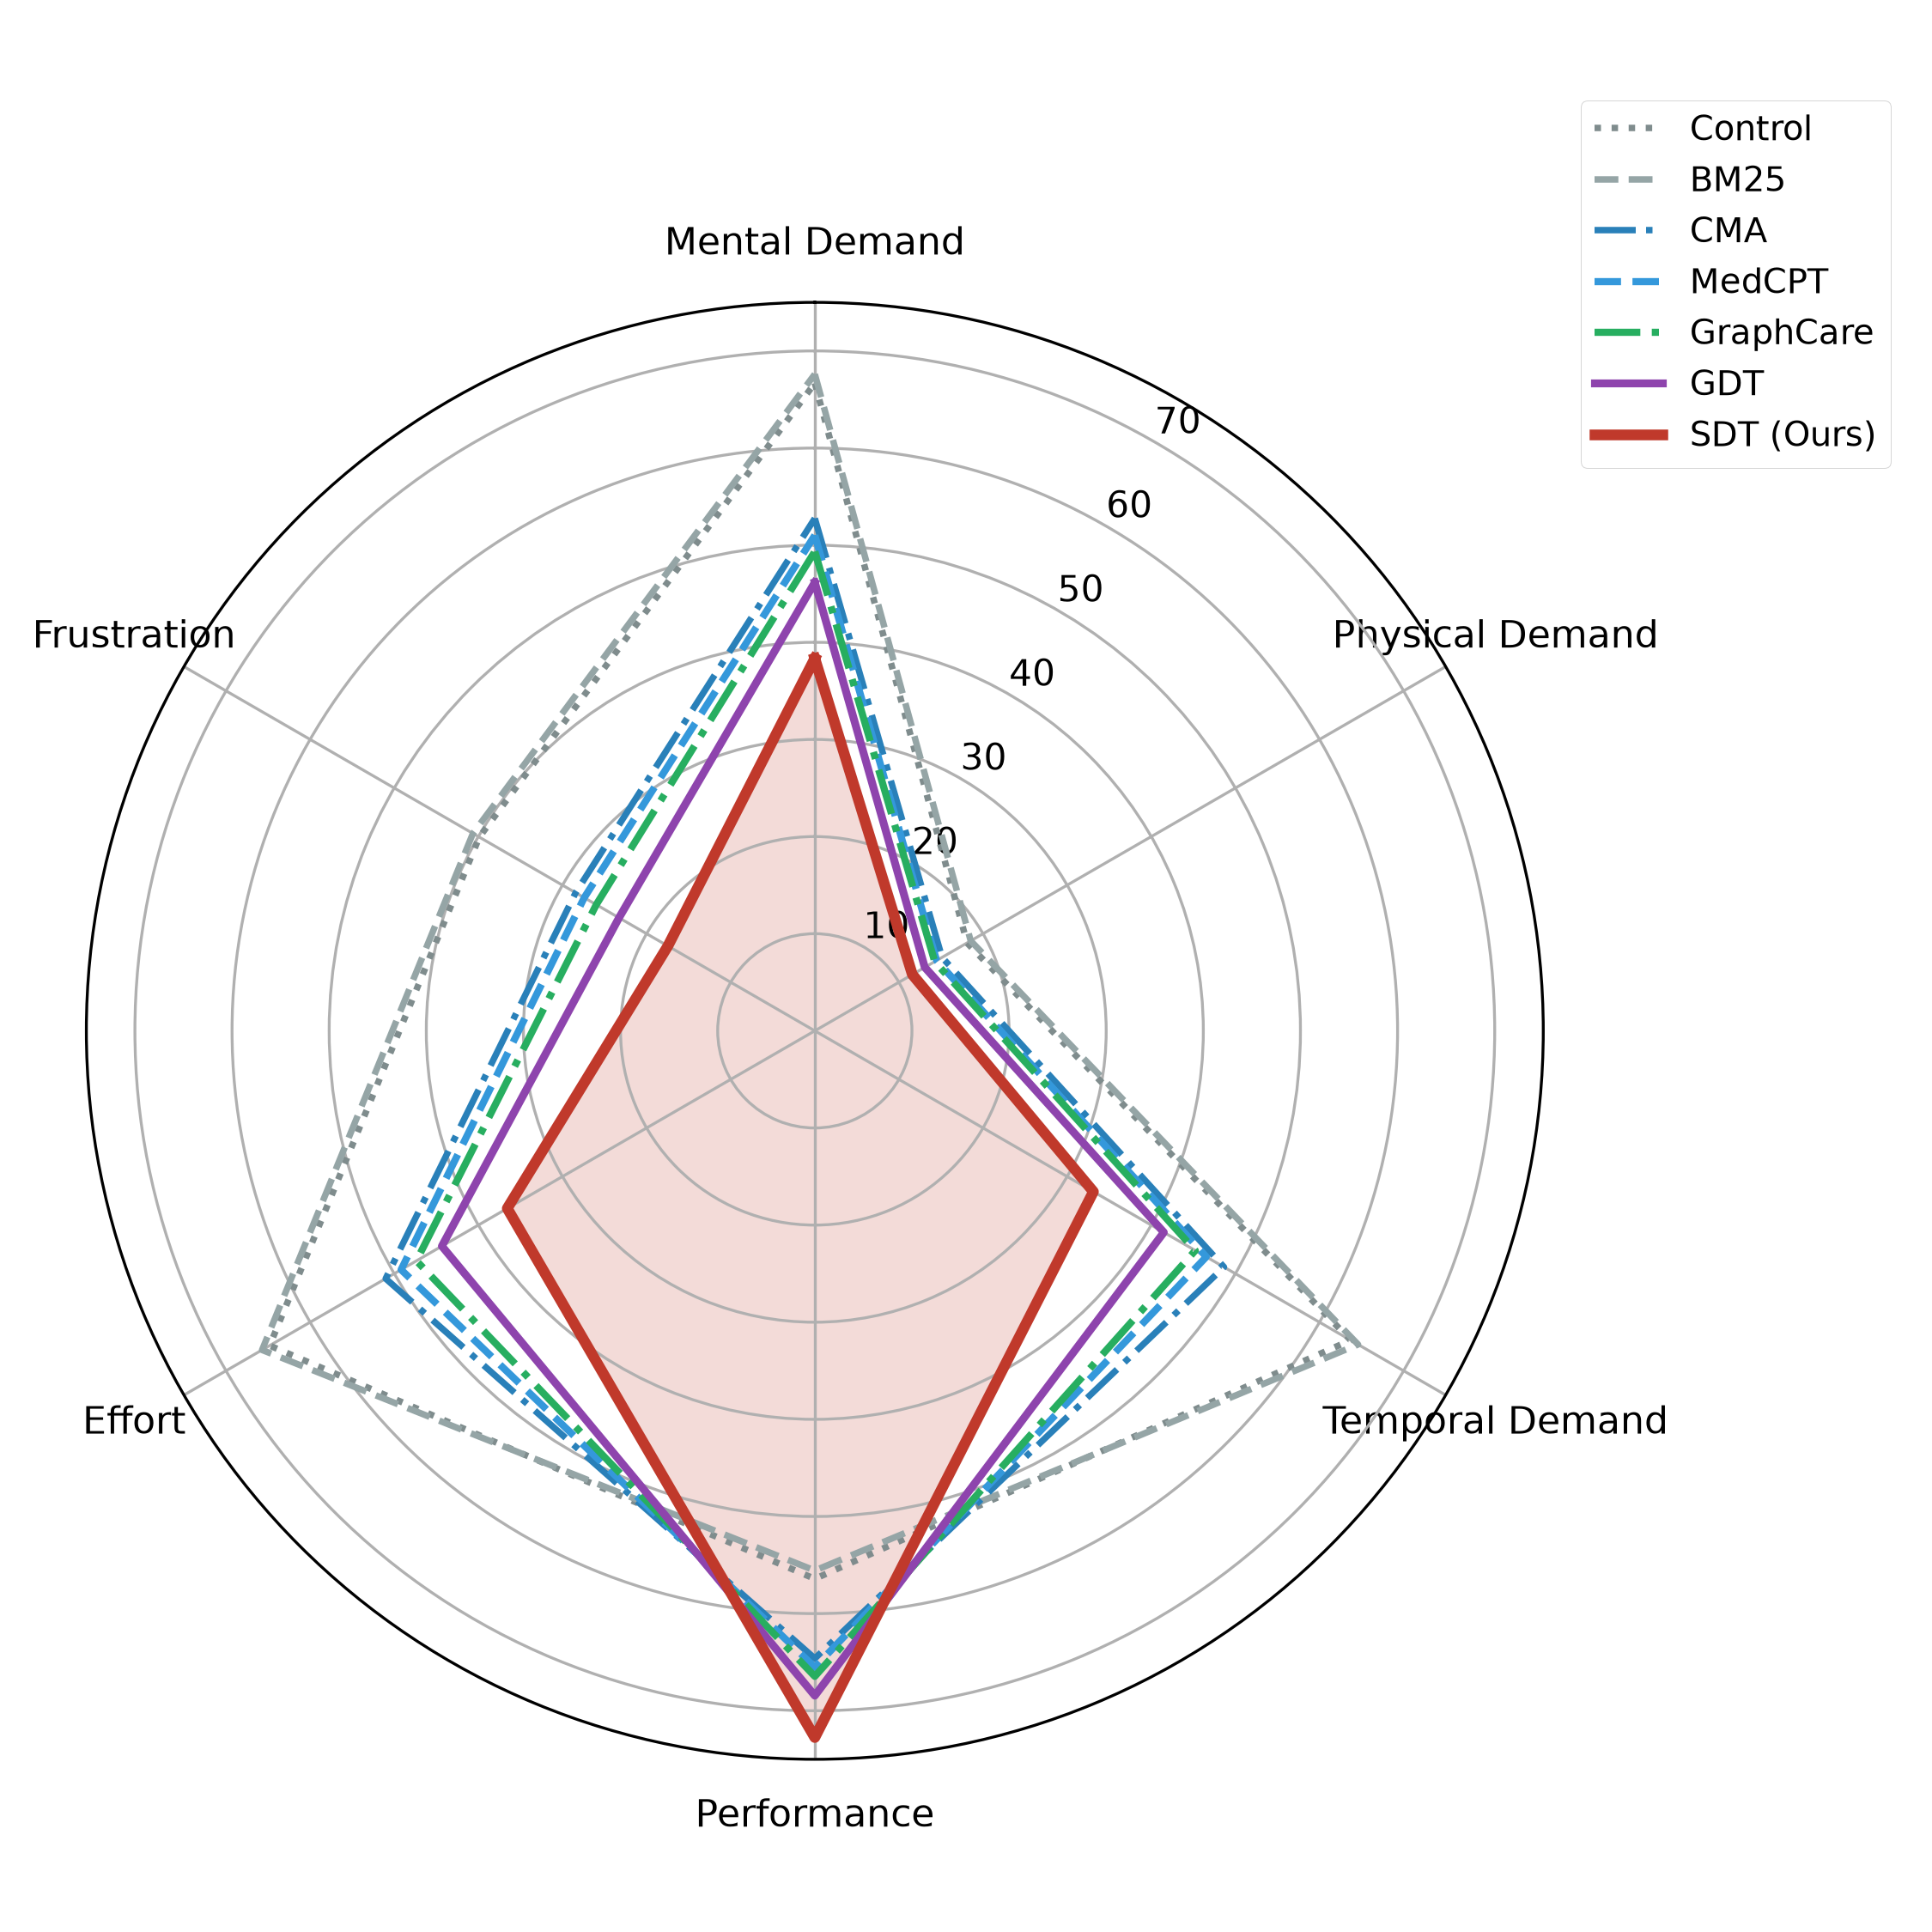
\includegraphics[width=0.40\textwidth]{fig_nasa_tlx_radar.png}\qquad
  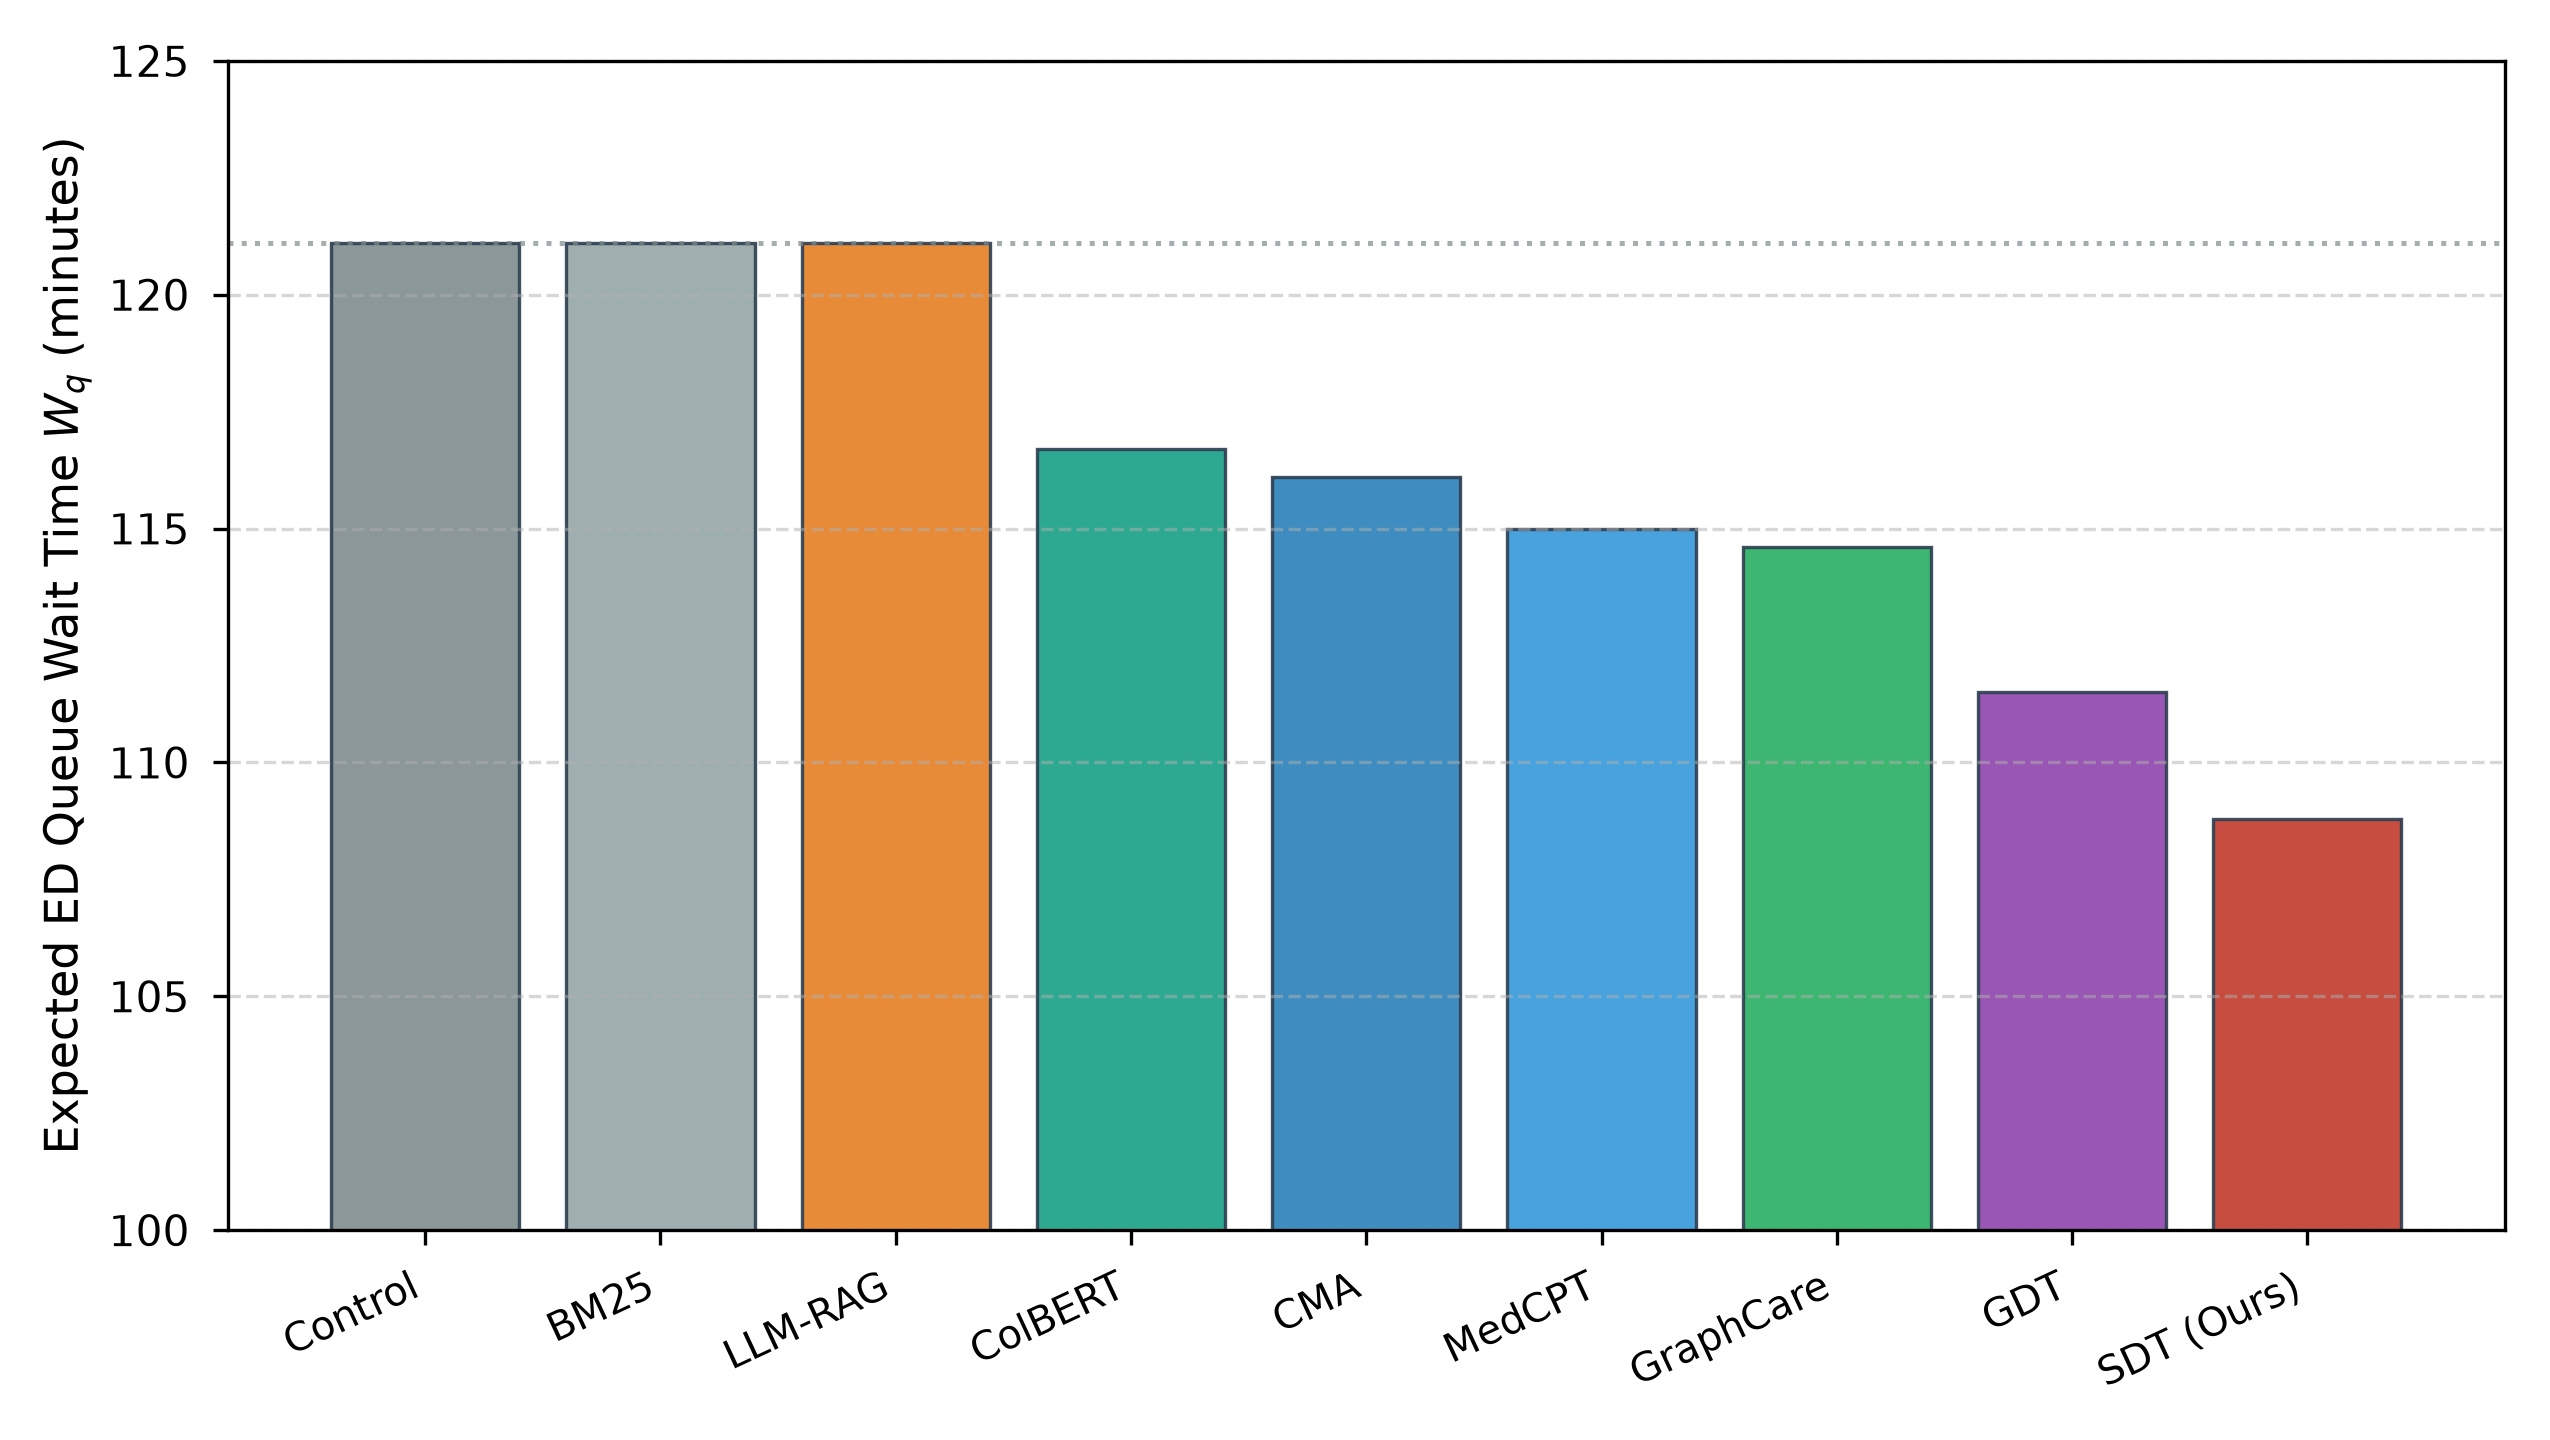
\includegraphics[width=0.48\textwidth]{fig_queueing_impact.png}
  \caption{(Left) NASA-TLX workload dimension profiles across retrieval paradigms; SDT demonstrates the lowest overall workload footprint. (Right) Projected emergency department patient queue waiting time ($W_q$) under Erlang C queueing modeling ($c=8, \lambda=6.0\,\text{hr}^{-1}, \mu=0.80\,\text{hr}^{-1}$), demonstrating super-linear operational leverage near queue saturation.}
  \label{fig:operational_impact}
\end{figure}

\subsection{Operational Queueing Translation}
We translated the 25.6-second per-encounter savings into an Erlang~C ($M/M/c$) queueing model of an Emergency Department staffed by $c = 8$ physicians with arrival rate $\lambda = 6.0\,\text{hr}^{-1}$ ($0.001667\,\text{s}^{-1}$) and baseline service rate $\mu = 0.80\,\text{hr}^{-1}$ ($1/\mu = 75.0$\,min/patient), operating at $\rho = 0.9375$ (93.75\% utilization). Per-patient chart review time savings $\Delta t$ accelerate the effective service rate to $\mu' = 1 / (4{,}500 - \Delta t)$, updating traffic intensity to $\rho' = \lambda / (c \mu')$. The steady-state probability of waiting $P_W$ and expected queue wait time $W_q$ are:
\begin{equation}
  P_W = \frac{\frac{(c \rho')^c}{c!(1-\rho')}}{\sum_{k=0}^{c-1} \frac{(c \rho')^k}{k!} + \frac{(c \rho')^c}{c!(1-\rho')}}, \quad W_q = \frac{P_W}{c \mu' (1 - \rho')}.
  \label{eq:erlang_c}
\end{equation}
Because queue delay scales as $(1-\rho')^{-1}$ near capacity, marginal sensitivity exhibits super-linear leverage: $\partial W_q / \partial(\Delta t) \approx \mathcal{O}((1-\rho)^{-2})$. As reported in Table~\ref{tab:queueing_results} and Figure~\ref{fig:operational_impact} (right), recovering 25.6\,s per encounter increases service rate from 0.8000 to 0.8046\,patients/hr—a 0.6\% throughput gain that yields an estimated 12.31-minute reduction in average patient queue wait time (121.10 to 108.79\,min). For an institution managing 50{,}000 emergency admissions annually, this eliminates over 10{,}200 hours of cumulative waiting room boarding.

% =============================================================================
\section{Clinical Vignette Walkthrough}
\label{sec:case_study}

To illustrate runtime mechanics, we trace a simulated high-complexity encounter (Vignette V260) involving an acute pivot. A 68-year-old male with COPD presents with fever (38.8$^\circ$C), productive cough, and right-sided pleuritic chest pain.

At $t=1$, the clinician queries ``sputum culture Gram stain,'' retrieving Gram-positive diplococci ($v_2$); hyperedge $e_1 = \{v_1, v_2\}$ yields $\lambda_2(L_1) = 1.00$. At $t=2$, querying ``prior chest radiograph consolidation'' ($v_3$) confirms right lower-lobe infiltrates. Semantic affinity across $\{v_1, v_2, v_3\}$ maintains high connectivity ($\lambda_2(L_2) = 0.88$), corroborating pneumonia.

At minute 28, telemetry alarms: the Mamba waveform encoder detects acute right ventricular strain (S1Q3T3 morphology, HR 88 to 132\,bpm, SpO$_2$ 86\%). The physician urgently queries ``D-dimer trend lower extremity Doppler.'' SDT ingests event node $v_4$ (D-dimer $>5{,}000\,\text{ng/mL}$) and telemetry node $v_5$. Because $\{v_4, v_5\}$ share negligible affinity with $\{v_1, v_2, v_3\}$, the graph bifurcates: $\lambda_2$ plunges from $0.88$ to $0.12$. Since $\Delta \lambda_2 = 0.76 > \tau_{\text{pivot}} = 0.15$, the Spectral Interference Gate triggers immediately.

Upon gate trigger, Chebyshev filter $H(L_3)$ attenuates background signals, and Fiedler vector coordinates $v_2 = [-0.48, -0.52, -0.44, +0.38, +0.40]^\top$ cleanly partition obsolete pneumonia nodes ($v_2 < 0$) from emergent PE nodes ($v_2 \ge 0$). Boundary hyperedges are severed, bounding context leakage below $\tau_{\text{pivot}} = 0.15$ (Theorem~\ref{thm:cheeger_bound}). Random walks over $G_{\text{global}}$ seeded from $\{v_4, v_5\}$ populate candidates with CT pulmonary angiogram protocols ($v_{101}$) and enoxaparin nomograms ($v_{102}$). Under cognitive budget $C_{\max} = 7.0$\,bits, both candidates are cached ($H=3.5 \le 7.0$). When the clinician searches for ``heparin contraindications,'' the dosing nomogram surfaces in $<15$\,ms, resolving the workup in 48.2\,s.

% =============================================================================
\section{Discussion}
\label{sec:discussion}

\paragraph{Topological Guarantees versus Manifold Smoothing.}
The advantage of SDT over GDT stems from how each models clinical reasoning. GDT conceptualizes intent as a smooth trajectory on an SPD covariance manifold. However, acute events are predominantly discrete: a lab breaches a threshold, telemetry exhibits sudden ischemic morphology, or imaging disproves an initial assumption. Forcing discrete shifts into continuous Riemannian metrics requires smoothing parameters that lag behind rapid pivots. In contrast, sparse hypergraphs accommodate discrete node additions and structural bisections natively: when disconnected evidence arrives, algebraic connectivity drops instantaneously, executing an exact Cheeger cut without smoothing latency.

\paragraph{Operational Boundaries and Limitations.}
SDT is specialized for complex multi-turn encounters and is not optimal across all retrieval regimes: (1)~\textbf{Factual Lookups}: For isolated single queries (e.g., blood type), hypergraph tracking adds $\sim$70\,ms overhead; standard BM25 remains optimal. (2)~\textbf{Low-Complexity Encounters}: In uncomplicated presentations without diagnostic pivots, $\Delta \lambda_2$ never breaches $\tau_{\text{pivot}}$, and SDT functions primarily as an anticipatory cache with performance comparable to dense bi-encoders. (3)~\textbf{Cold-Start Facilities}: Anticipatory prefetching relies on precomputed Laplacian eigenspaces of historical records ($G_{\text{global}}$); sparse databases must accumulate interaction history before enabling spectrally biased walks.

\paragraph{Clinical Safety, Automation Bias, and EHR Deployment.}
Proactive retrieval risks automation bias: aggressively staging confirmatory documents could reinforce diagnostic tunnel vision \cite{goddard2012automation}. SDT mitigates this through its surprisal tax (Eq.~\eqref{eq:surprisal_cost}): speculative records far from the active hypothesis are heavily penalized, preventing cognitive clutter. Clinicians retain full ordering agency, and severed subgraphs can be restored with a single click. Deployment requires no EHR overhaul: standard SMART-on-FHIR protocols and \texttt{patient-view} CDS Hooks can instantiate hypergraph $G_t$ in a background service upon chart access, while continuous telemetry is ingested via HL7 observation streams and prefetched records are staged in an in-memory Redis cache to populate real-time autocomplete suggestions.

% =============================================================================
\section{Conclusion}
\label{sec:conclusion}

Spectral Diagnostic Trajectories (SDT) models active clinical workflows as evolving multi-modal hypergraphs. Tracking hypergraph algebraic connectivity ($\lambda_2$) detects diagnostic pivots in linear time, decouples obsolete context with formal Cheeger conductance bounds, and prefetches prospective records under working memory constraints. Across 1{,}000 diagnostic vignettes evaluated in a 9-arm simulation, SDT reduced retrieval time by 28.9\% versus standard search and by 8.7\% versus GDT, improving diagnostic accuracy to 93.9\% and cutting modeled cognitive load by 32.2\% at a mean latency of 112.9\,ms. Operational queueing modeling demonstrates super-linear throughput gains, eliminating an estimated 12.3 minutes of patient queue waiting time under near-saturation emergency conditions. Future work will focus on silent-mode prospective bedside trials.

% =============================================================================
\section*{Ethics Statement, Acknowledgements, and Disclosures}
\footnotesize
\noindent\textbf{Ethics Statement:} This study utilized exclusively de-identified, open-access databases (MIMIC-IV v2.2, MIMIC-CXR, HiRID) under PhysioNet Credentialed DUA \#481920 with institutional IRB oversight and HIPAA Safe Harbor compliance.
\textbf{Acknowledgements \& Funding:} The authors thank the MIMIC and PhysioNet curation teams. This research received no external financial support. The authors declare no competing financial or personal interests.

% =============================================================================
\begingroup
\scriptsize
\setlength{\bibsep}{0.6pt plus 0.2pt minus 0.1pt}
\begin{multicols}{2}
\bibliographystyle{unsrtnat}
\bibliography{references}
\end{multicols}
\endgroup

\end{document}
